\documentclass{article}
\usepackage{graphicx}
\usepackage{amsmath, amssymb}
\usepackage{hyperref}
\usepackage{booktabs}
\usepackage{subcaption} % For subfigures

\title{Seng 474 Assignment 3}
\author{Isaak Wiebe}
\date{March 17, 2025}

\begin{document}

\maketitle

\section{Introduction}
This report presents the results of clustering experiments performed using Lloyd’s algorithm (k-means) and hierarchical agglomerative clustering on two datasets. The objective is to analyze the clustering results and determine an appropriate number of clusters for each dataset.

\section{Algorithms and Implementation}
\subsection{Lloyd’s Algorithm (k-means)}
Two initialization methods were implemented:
\begin{itemize}
    \item Uniform random initialization
    \item k-means++ initialization
\end{itemize}
Euclidean distance was used to compute cluster assignments.

\subsection{Hierarchical Agglomerative Clustering}
Dissimilarity was measured using Euclidean distance. Both single linkage and average linkage clustering methods were applied. Dendrograms were generated for cluster selection.

\section{Datasets}
\begin{itemize}
    \item \textbf{Dataset 1}: 3500 two-dimensional examples generated using a Gaussian mixture model.
    \item \textbf{Dataset 2}: 14,801 three-dimensional examples.
\end{itemize}

\section{Experimental Results}
\subsection{Lloyd’s Algorithm Results}
For each dataset, multiple values of $k$ were tested, and the clustering cost was plotted against $k$. The optimal number of clusters was determined based on the elbow method.

\begin{figure}[h]
    \centering
    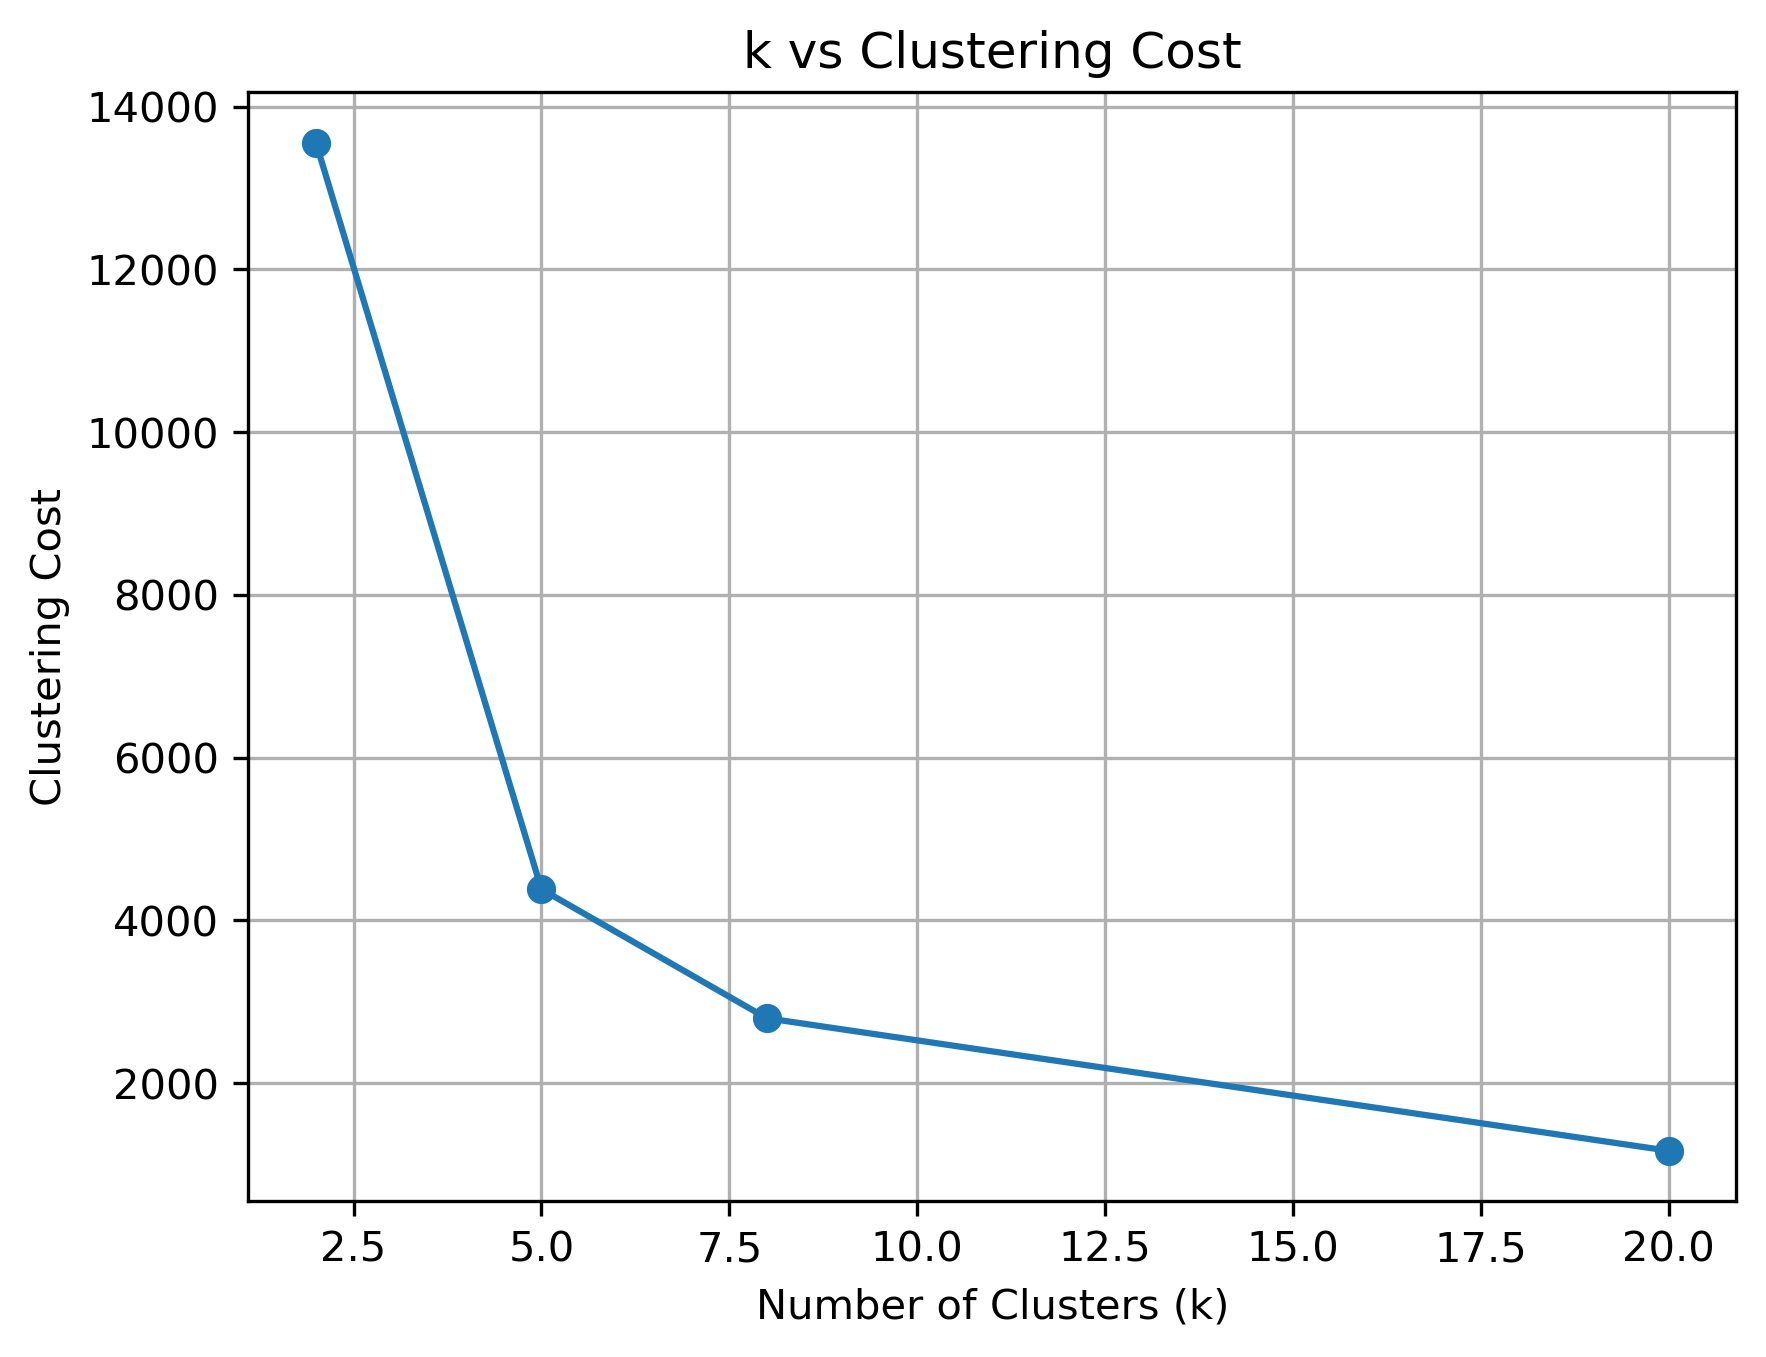
\includegraphics[width=0.7\textwidth]{figures/k_vs_cost0.png} % Replace with actual figure
    \caption{Clustering cost vs. number of clusters ($k$) for Dataset 1}
    \label{fig:cost_plot1}
\end{figure}

\begin{figure}[h]
    \centering
    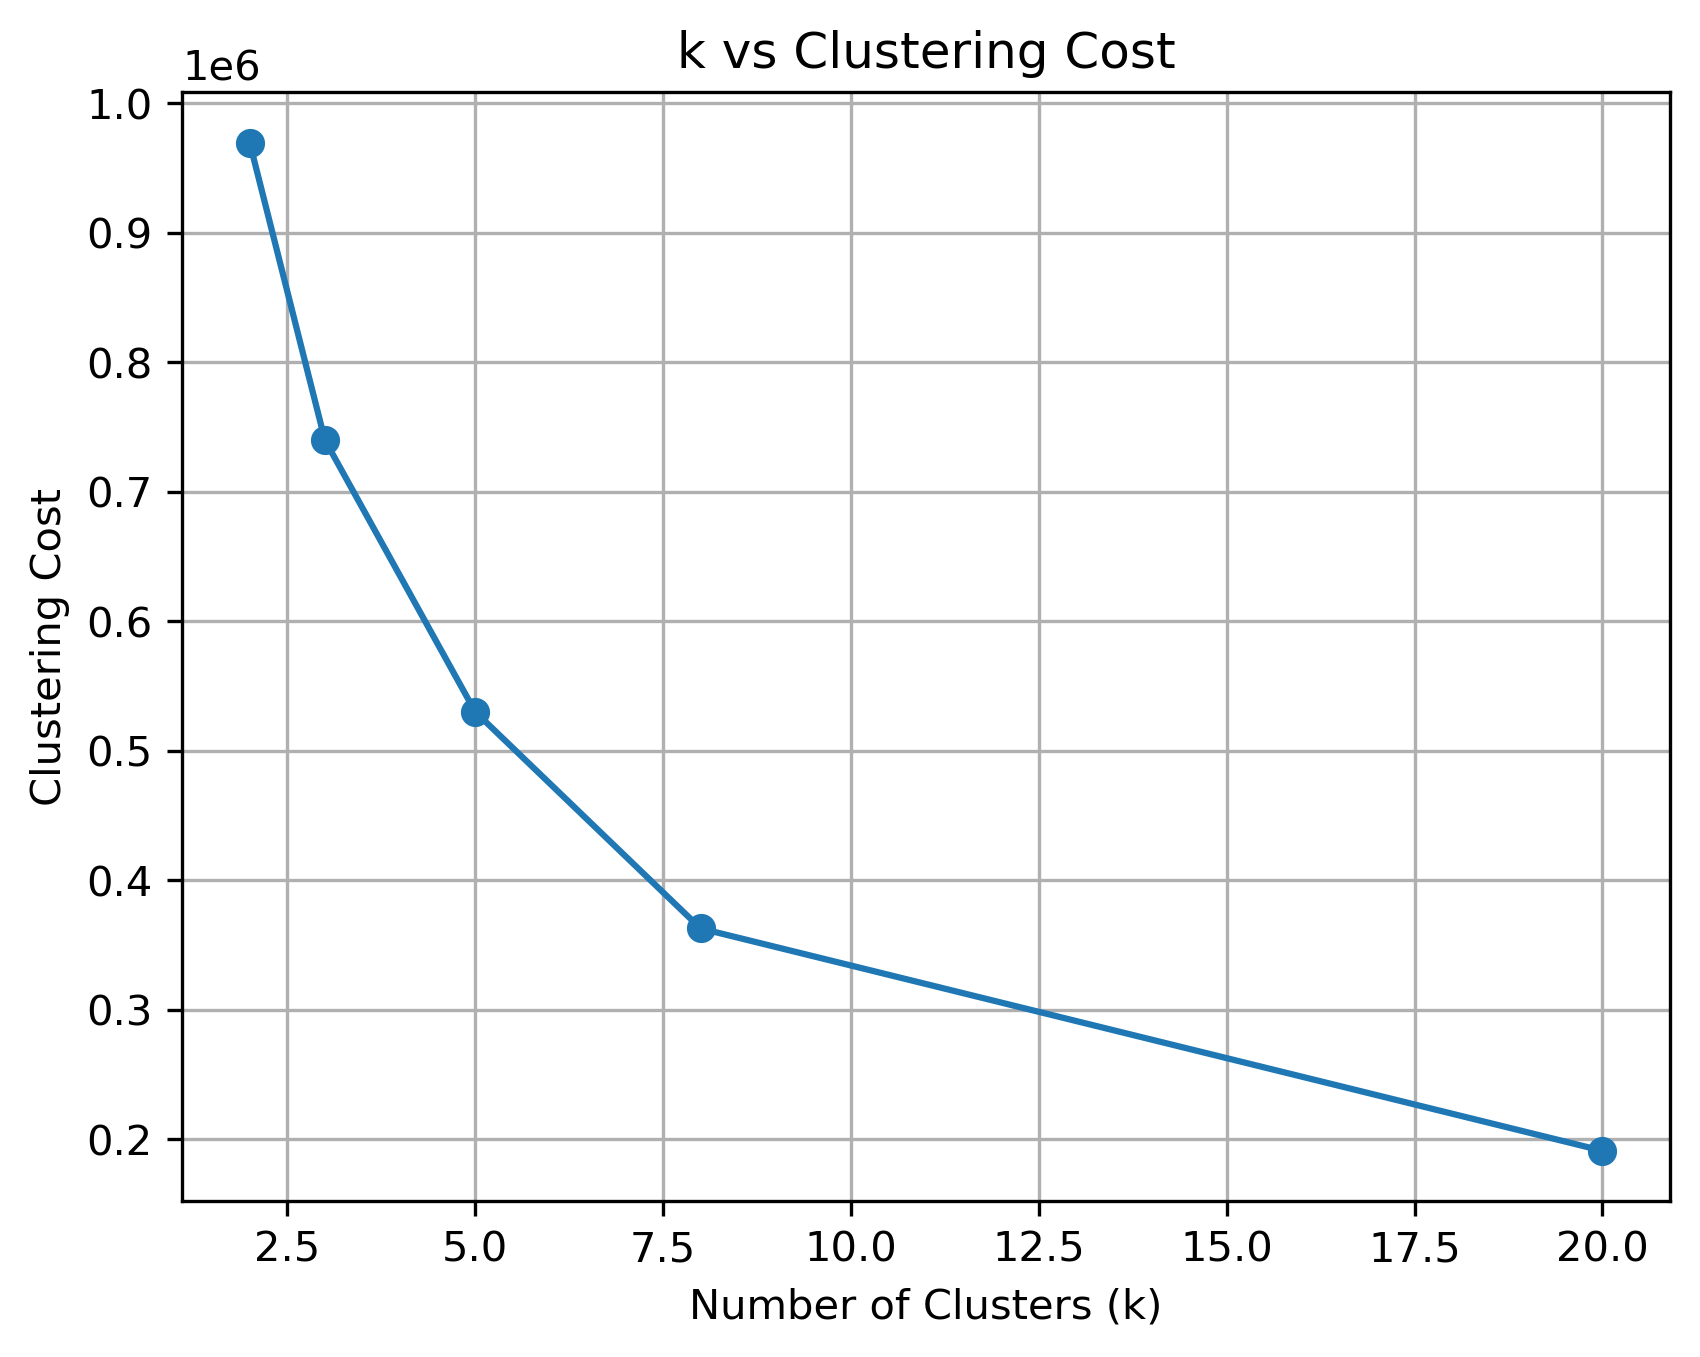
\includegraphics[width=0.7\textwidth]{figures/k_vs_cost1.png} % Replace with actual figure
    \caption{Clustering cost vs. number of clusters ($k$) for Dataset 2}
    \label{fig:cost_plot2}
\end{figure}

\subsection{Scatterplots for k-means Clustering}
The scatterplots for k-means clustering are shown below for both datasets. Each row corresponds to a dataset, and each column corresponds to a value of $k$.

\begin{figure}[h]
    \centering
    \begin{subfigure}[b]{0.45\textwidth}
        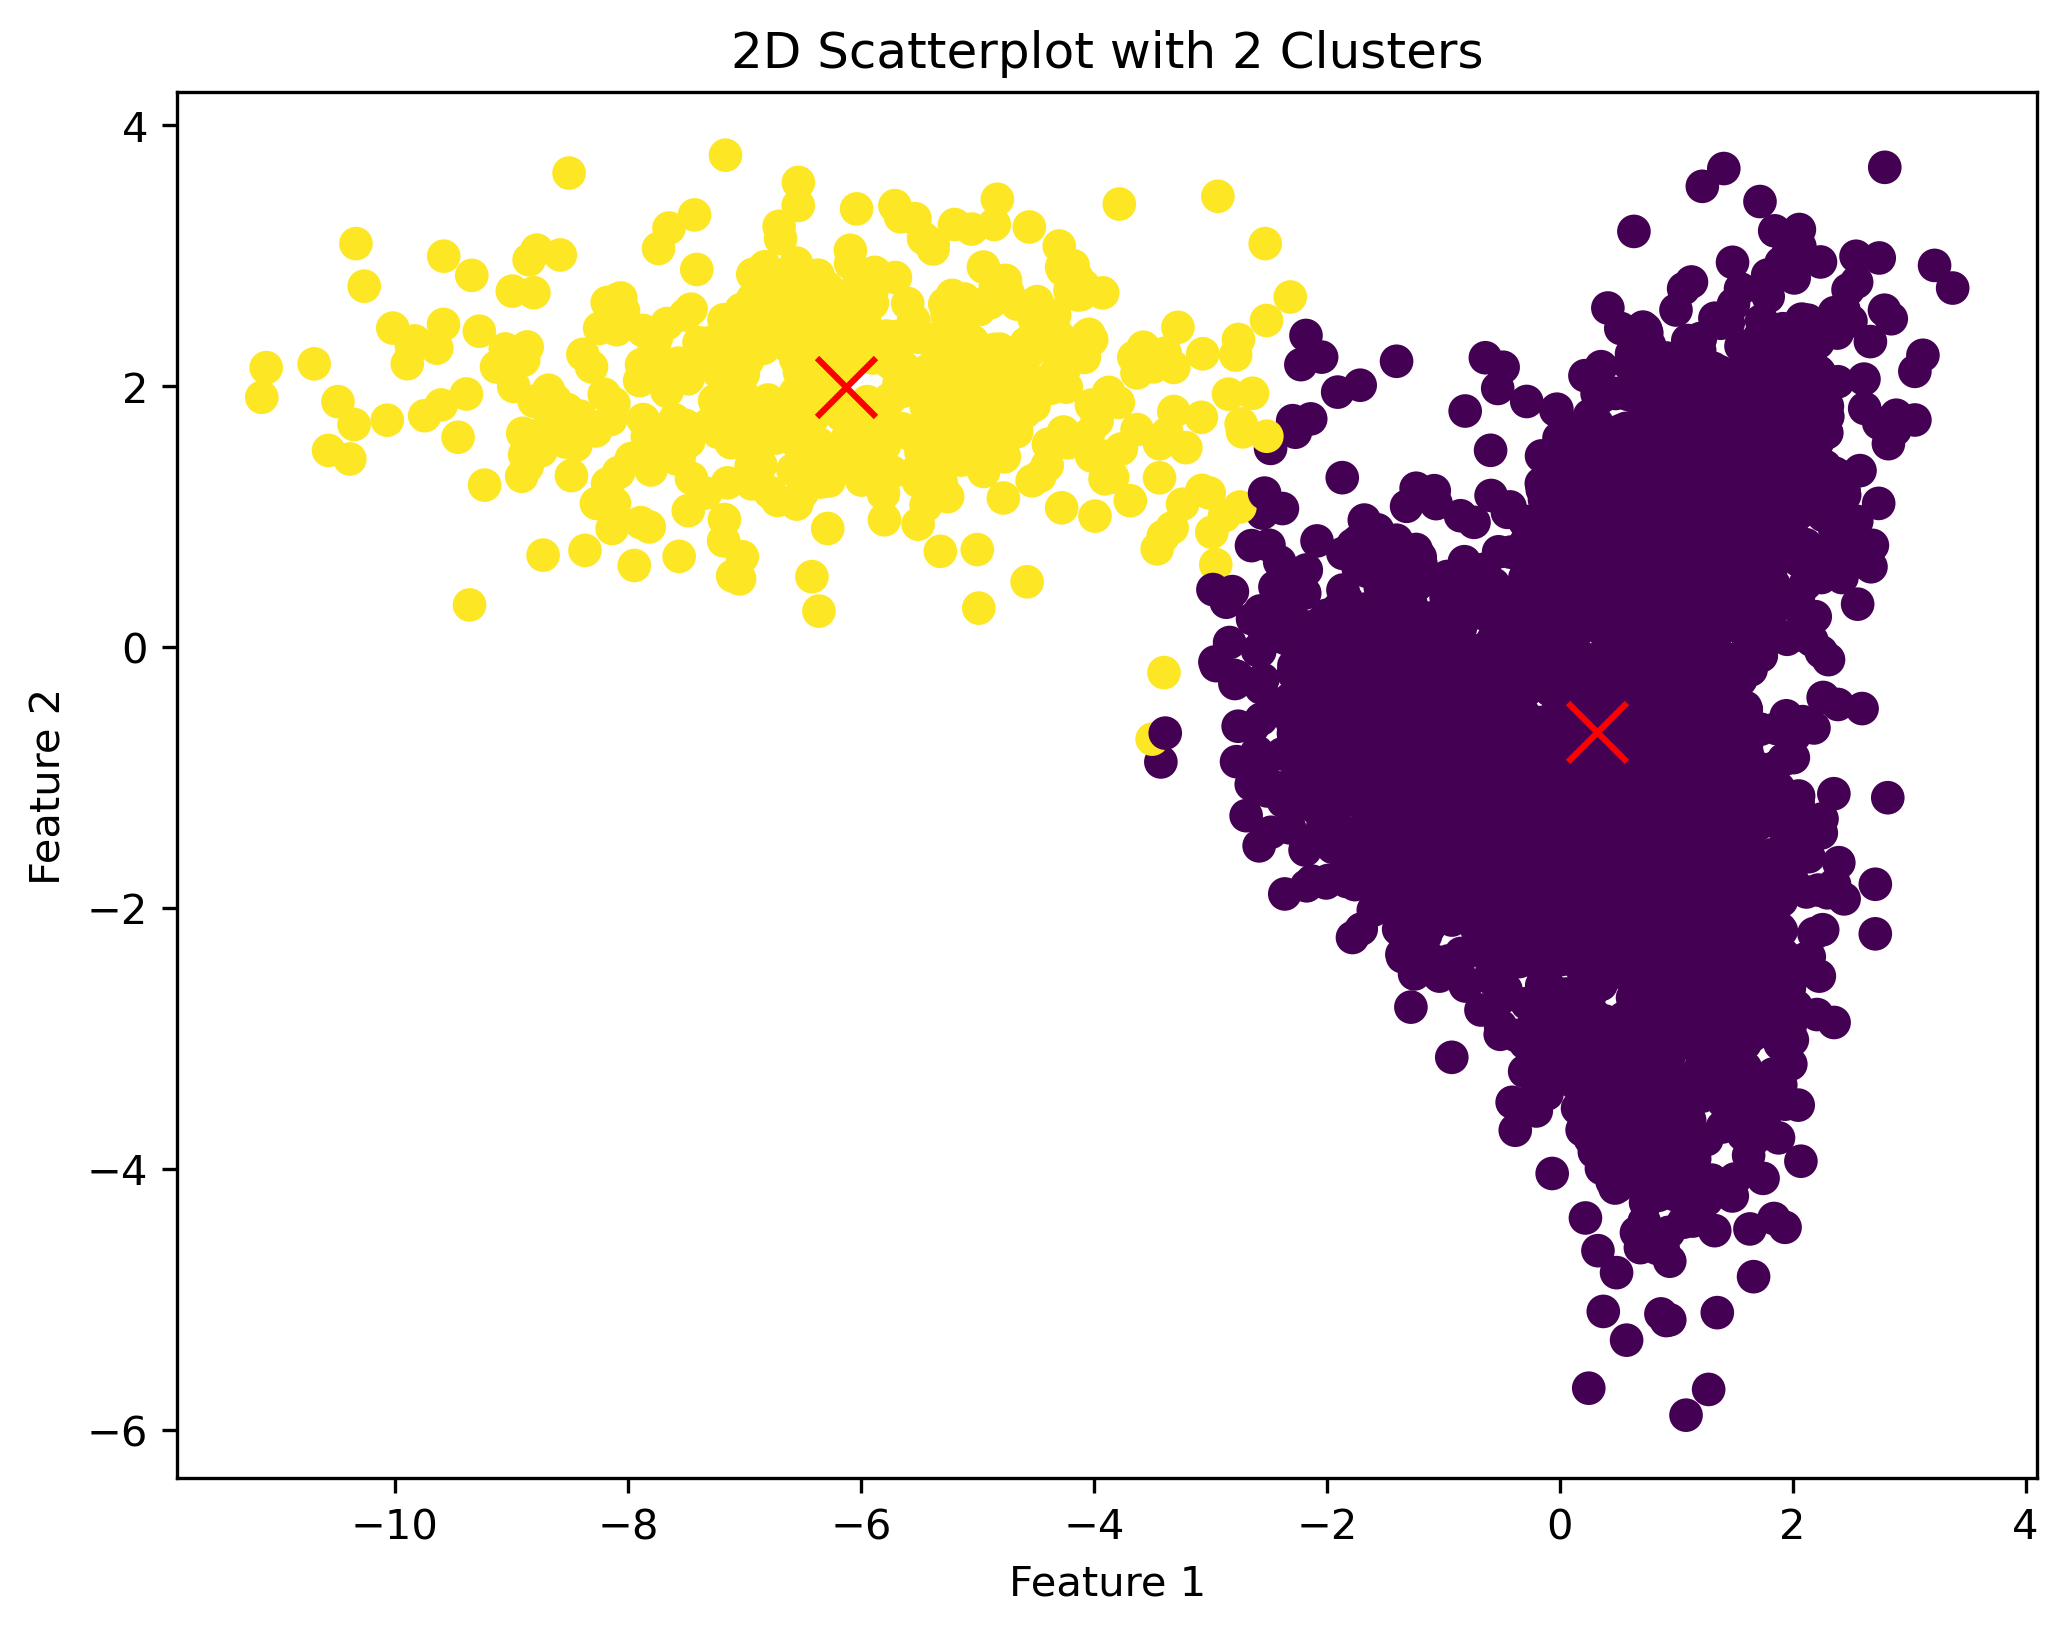
\includegraphics[width=\textwidth]{figures/2d_scatter_k2_d0.png}
        \caption{$k=2$ (Dataset 1)}
        \label{fig:2d_k2}
    \end{subfigure}
    \begin{subfigure}[b]{0.45\textwidth}
        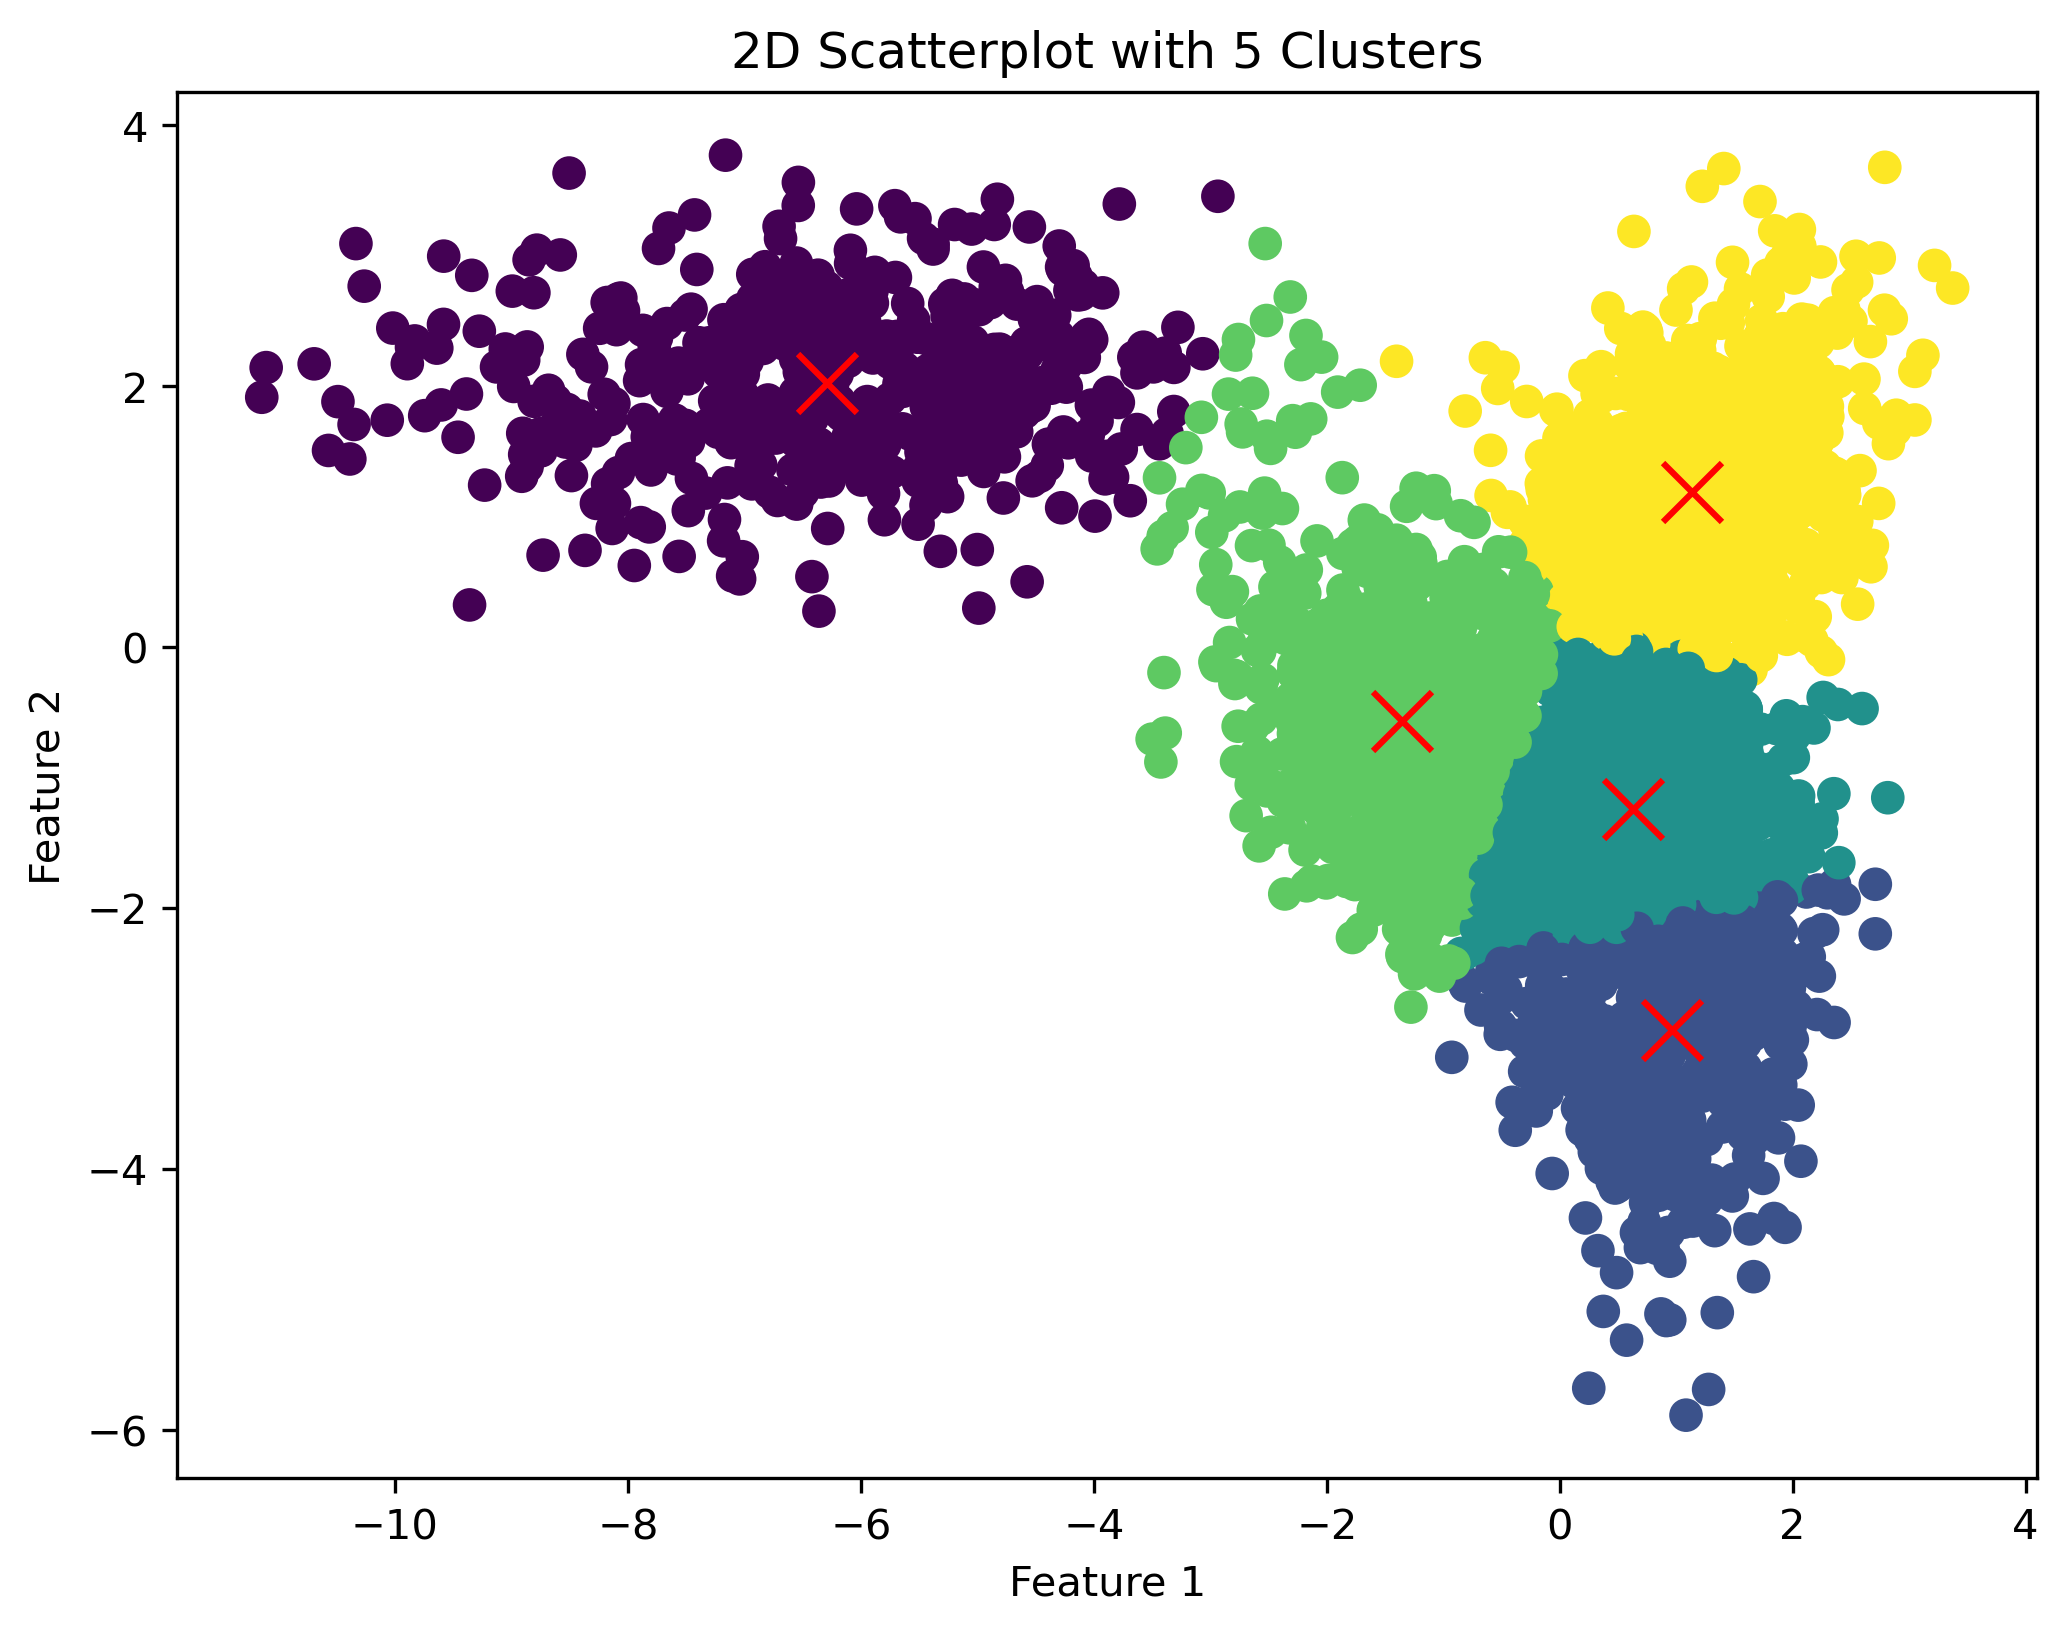
\includegraphics[width=\textwidth]{figures/2d_scatter_k5_d0.png}
        \caption{$k=5$ (Dataset 1)}
        \label{fig:2d_k5}
    \end{subfigure}
    \begin{subfigure}[b]{0.45\textwidth}
        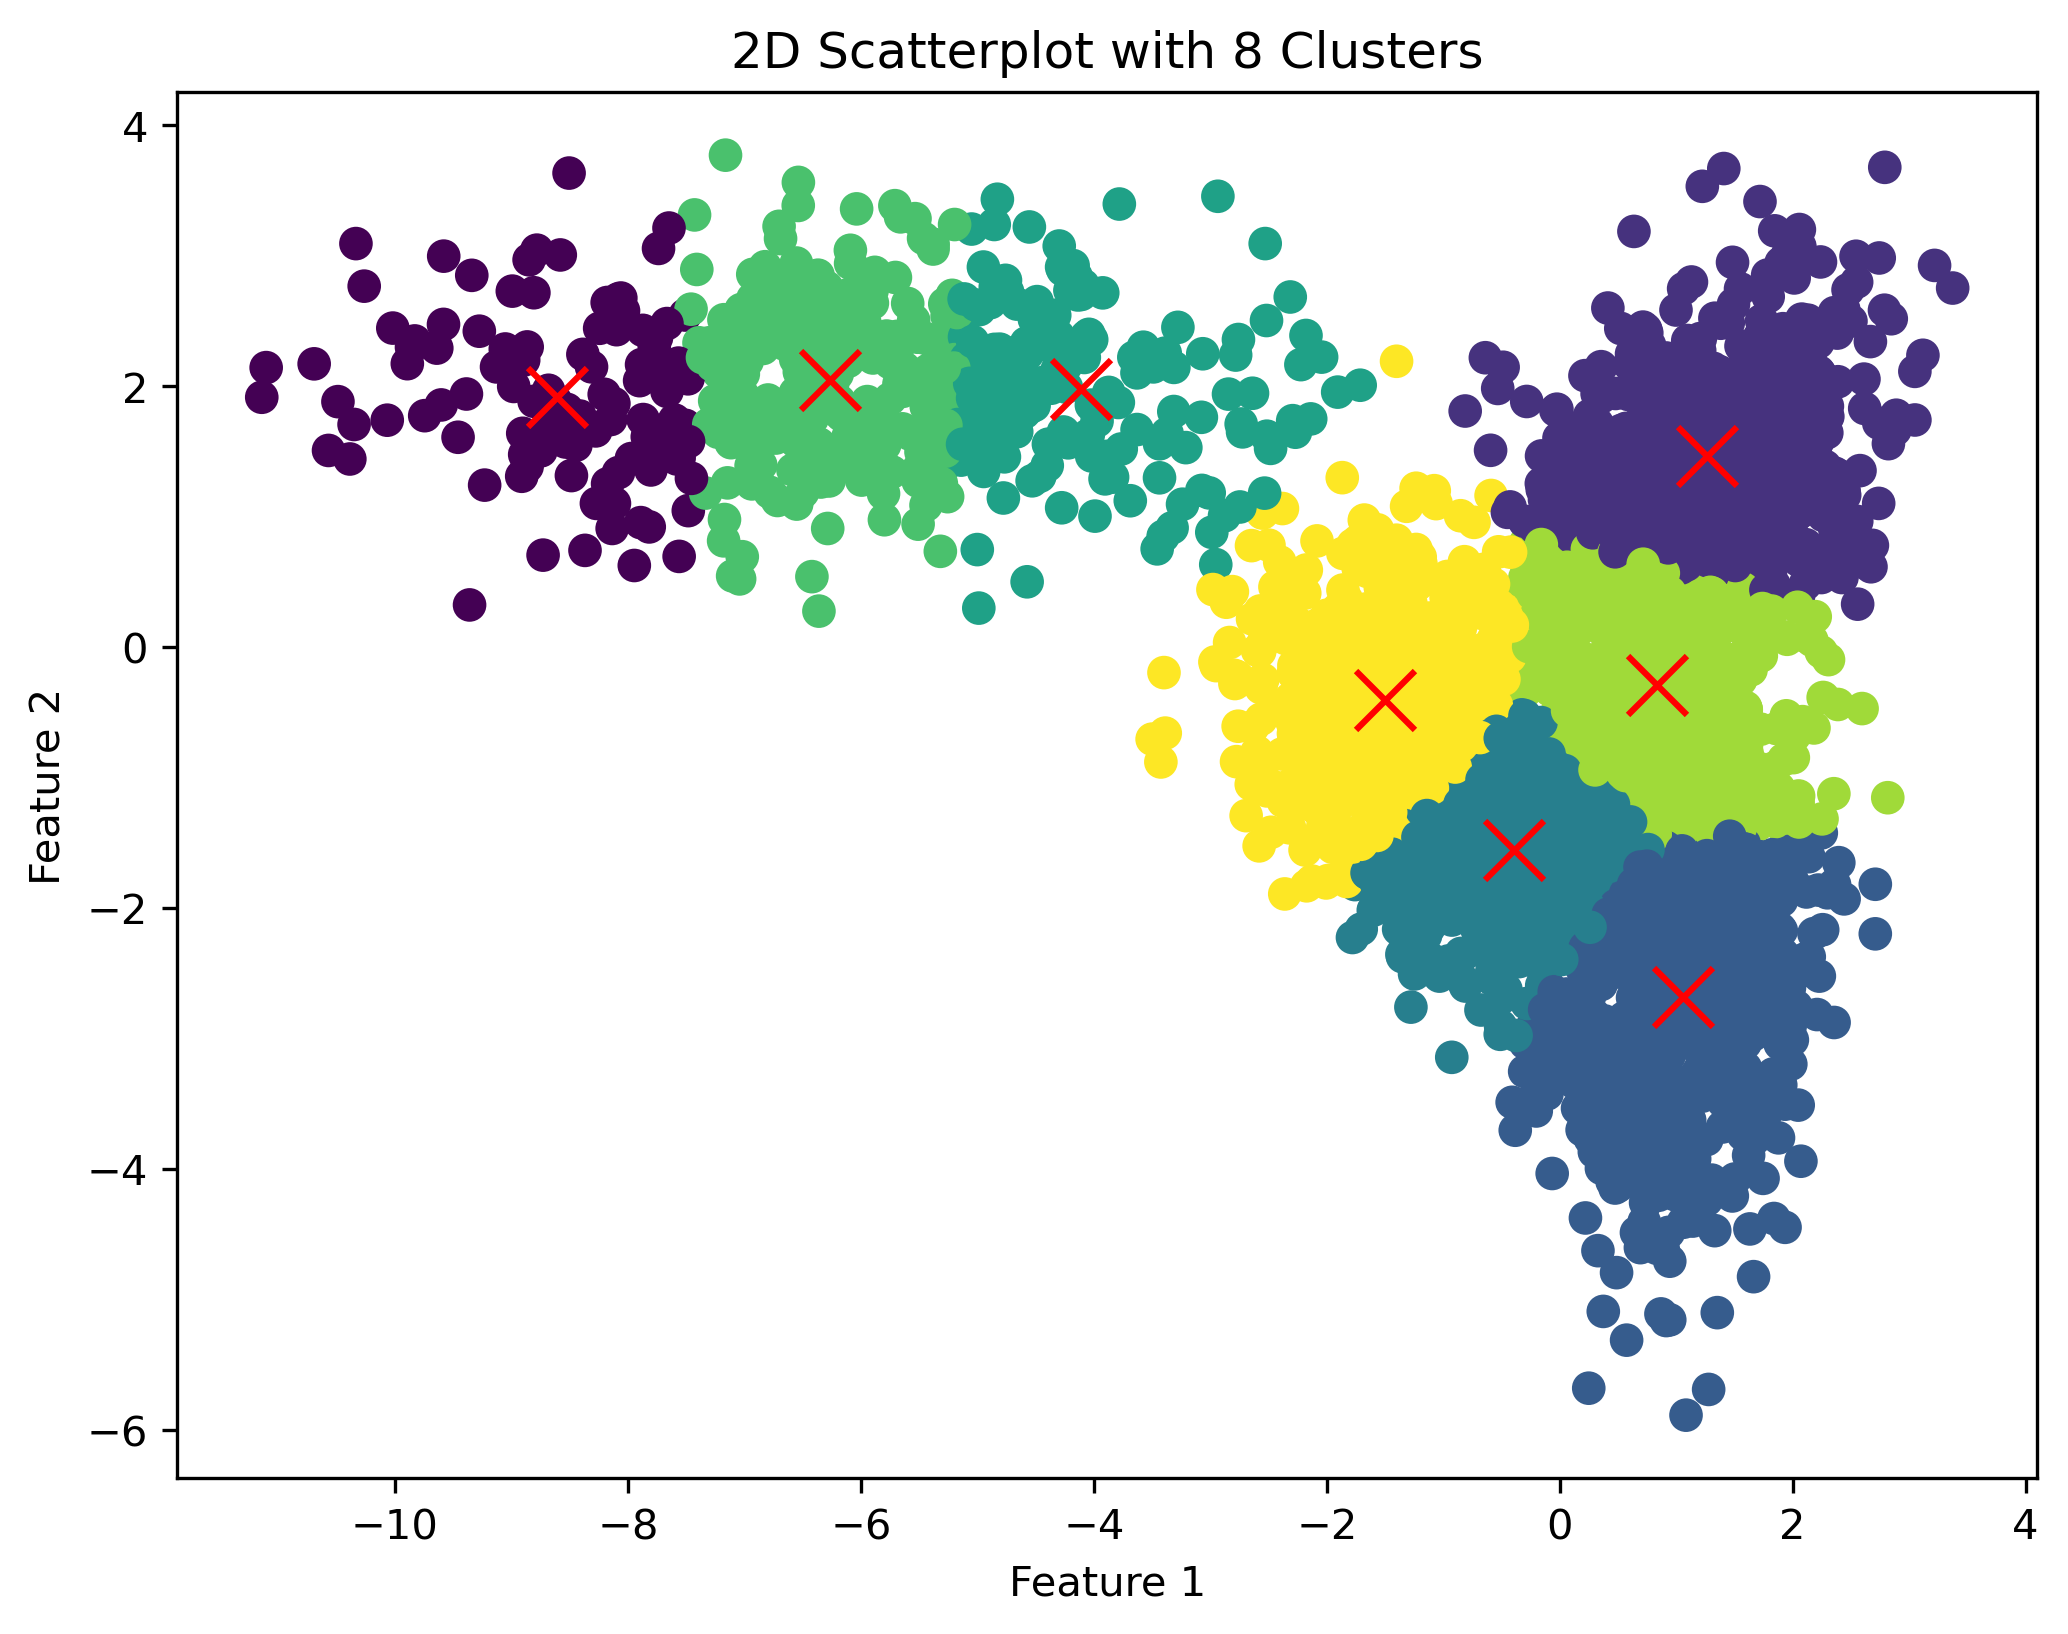
\includegraphics[width=\textwidth]{figures/2d_scatter_k8_d0.png}
        \caption{$k=8$ (Dataset 1)}
        \label{fig:2d_k8}
    \end{subfigure}
    \begin{subfigure}[b]{0.45\textwidth}
        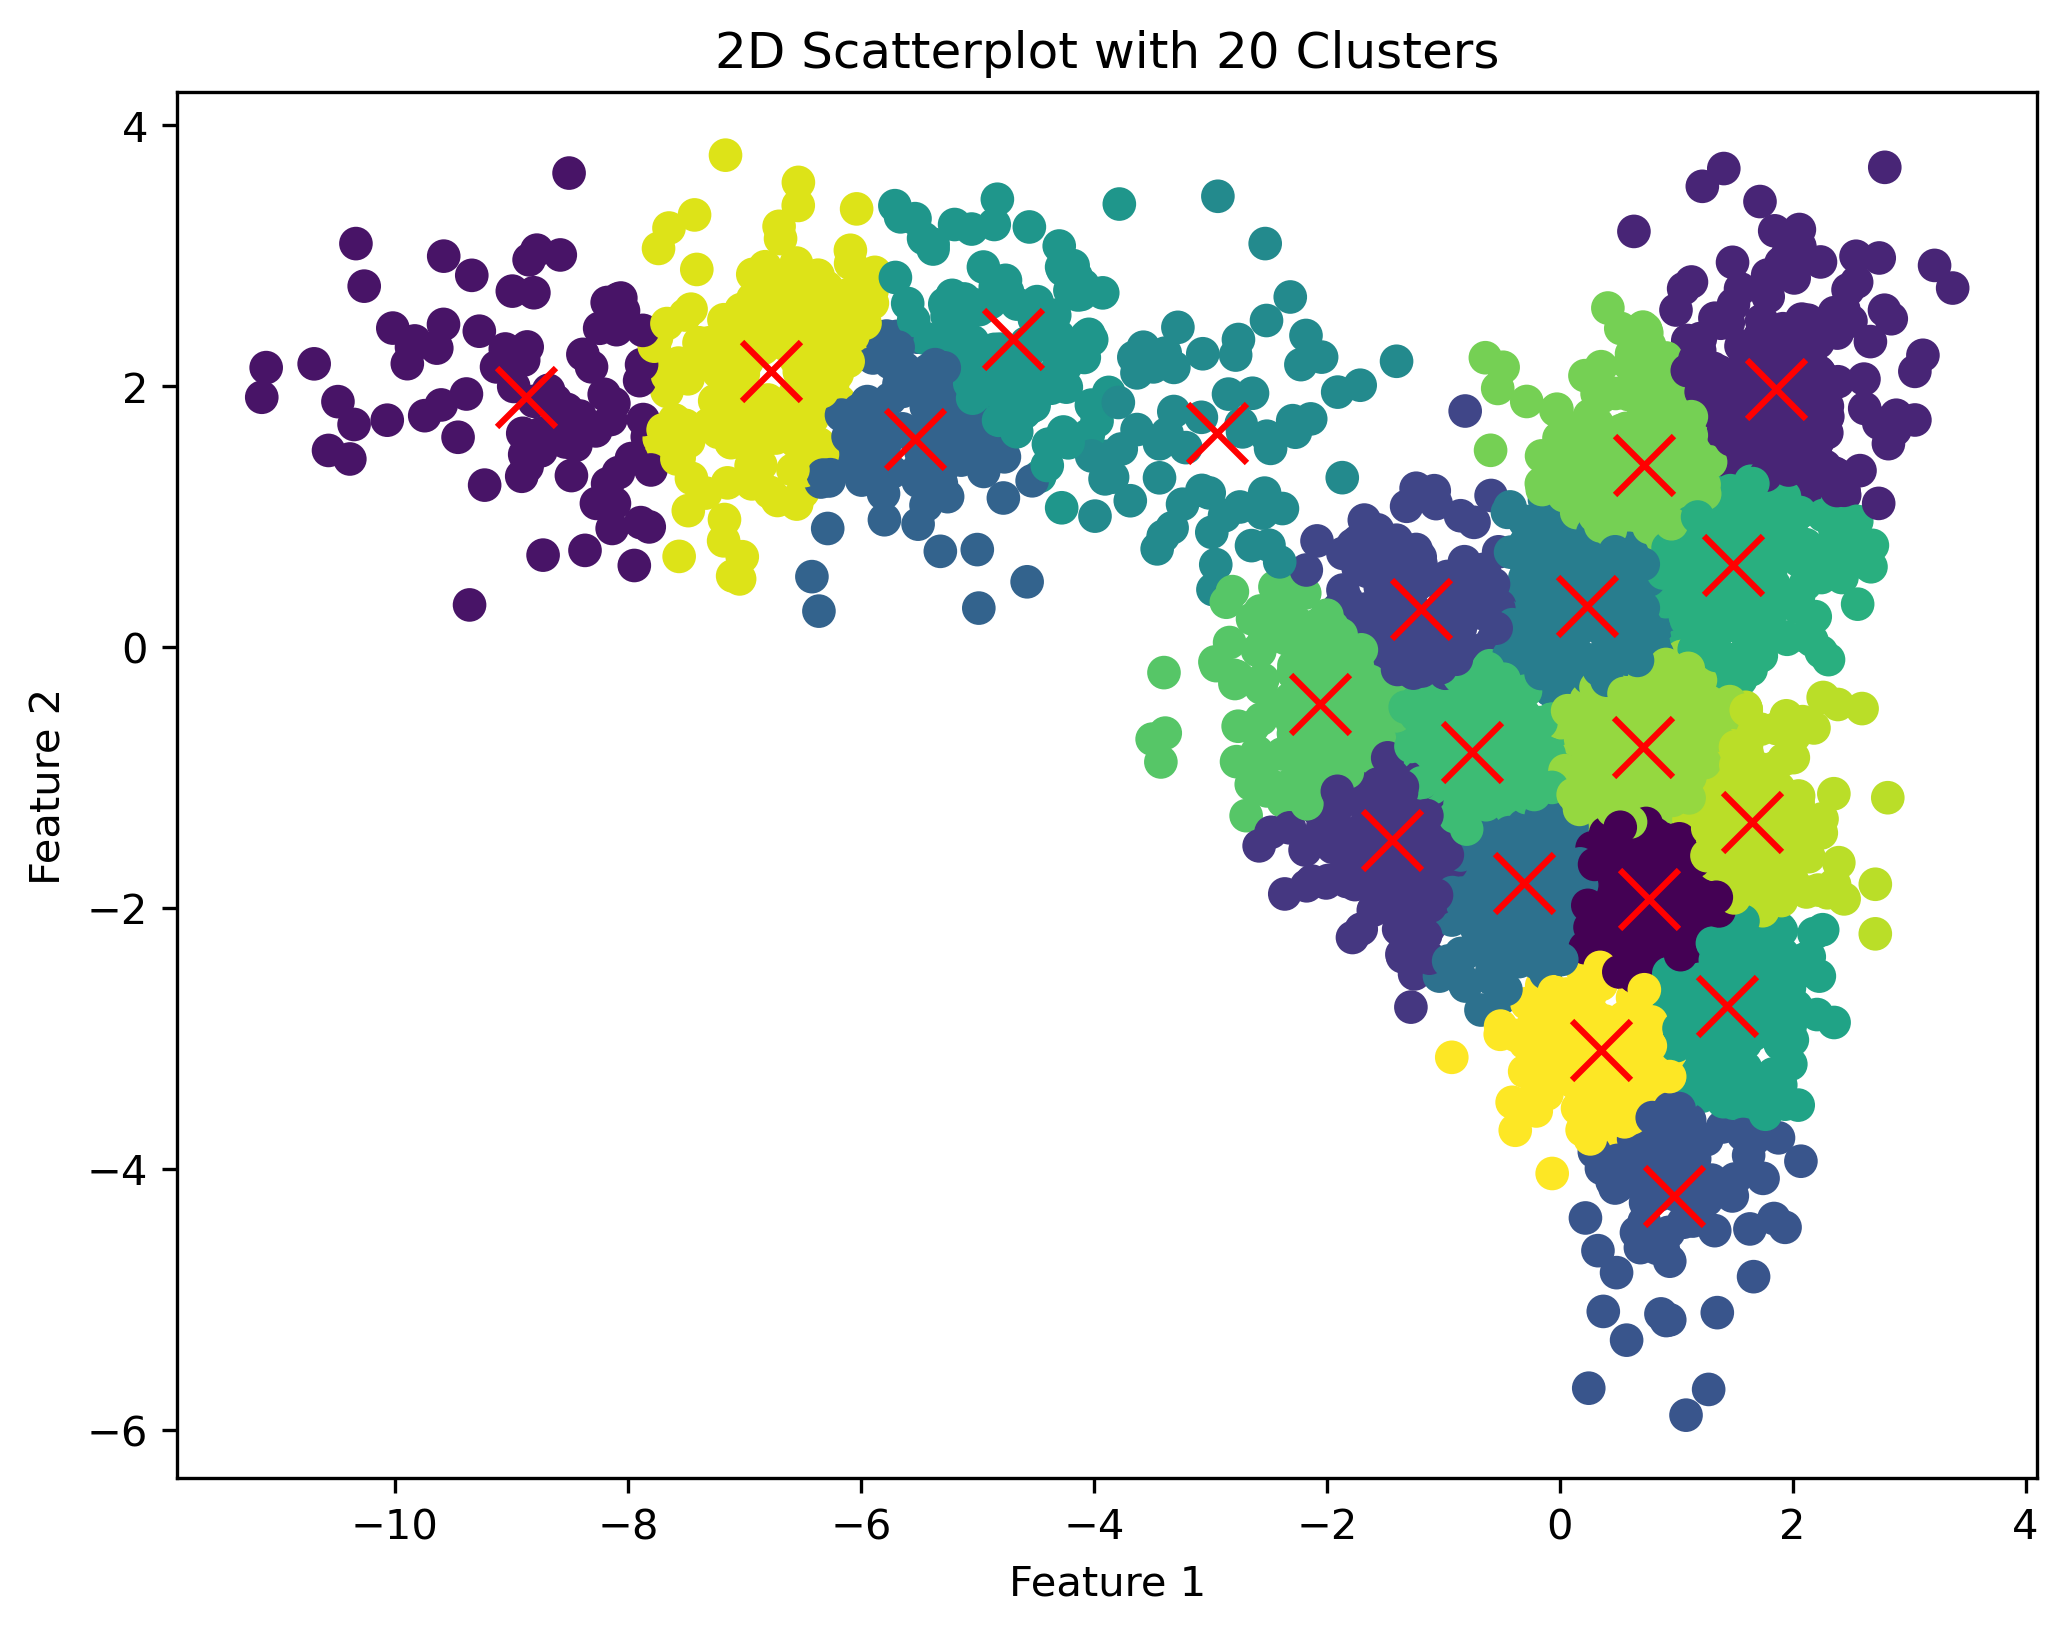
\includegraphics[width=\textwidth]{figures/2d_scatter_k20_d0.png}
        \caption{$k=20$ (Dataset 1)}
        \label{fig:2d_k20}
    \end{subfigure}
    \caption{Scatterplots for k-means with clustering k++ initialization on Dataset 1 (2D)}
    \label{fig:2d_scatterplots}
\end{figure}

\begin{figure}[h]
    \centering
    \begin{subfigure}[b]{0.45\textwidth}
        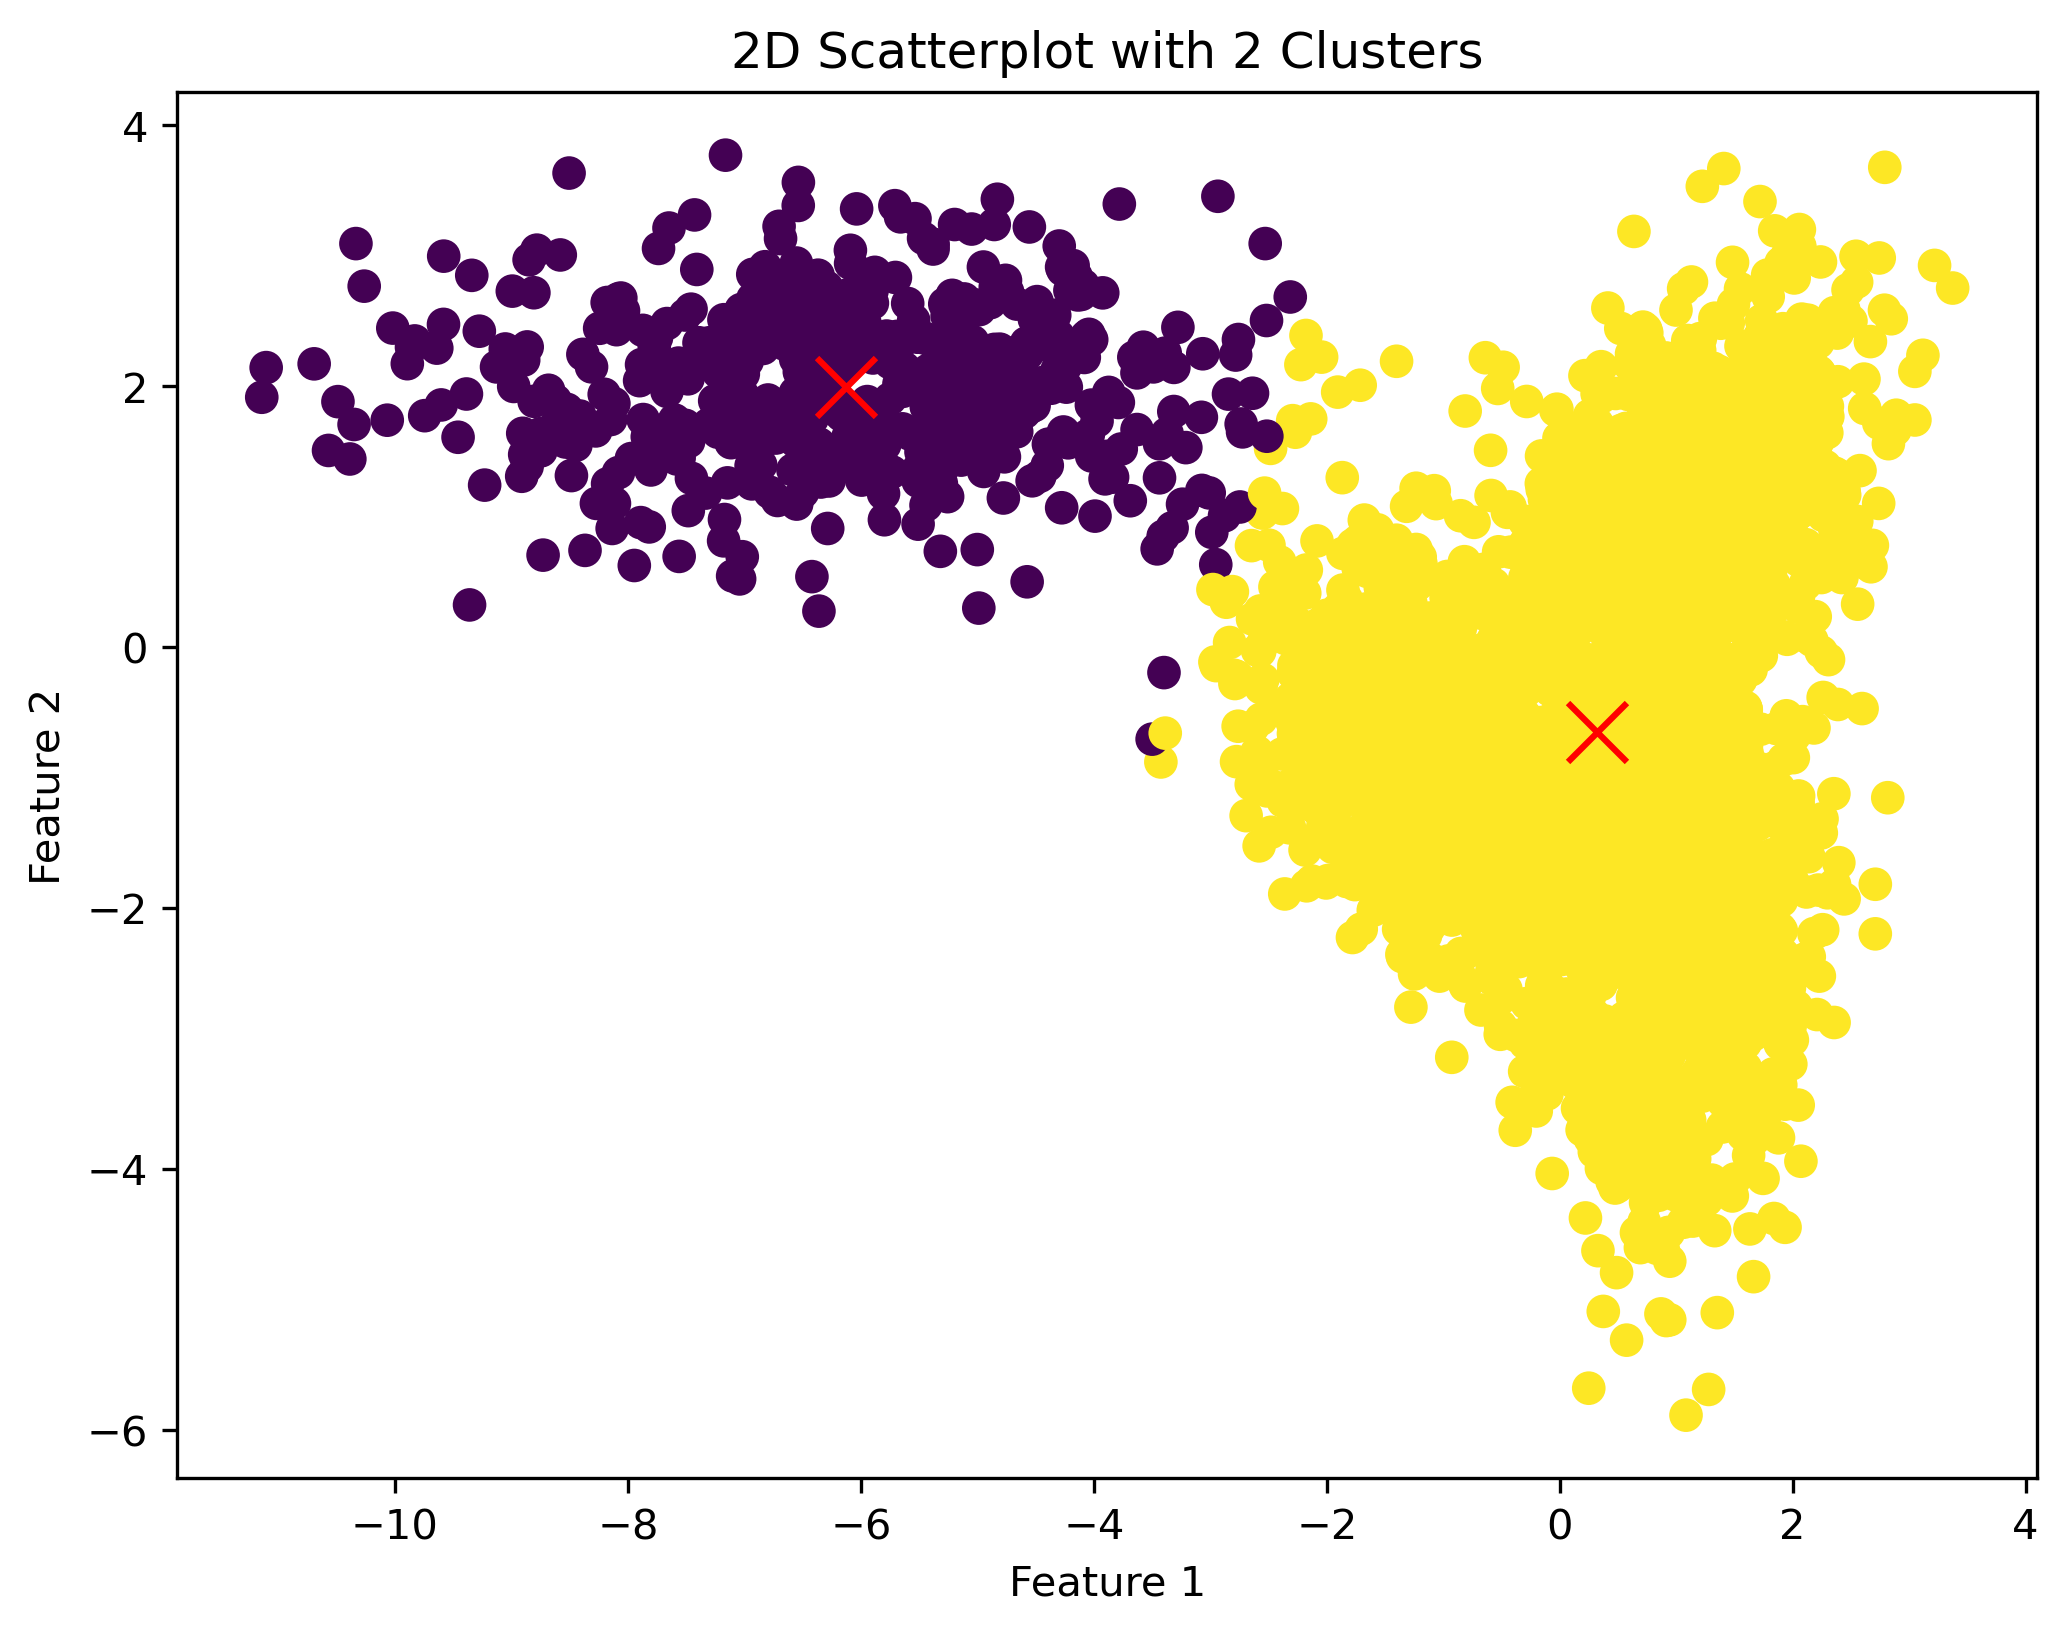
\includegraphics[width=\textwidth]{figures/random_2d_scatter_k2_d0.png}
        \caption{$k=2$ (Dataset 1)}
        \label{fig:2d_k2}
    \end{subfigure}
    \begin{subfigure}[b]{0.45\textwidth}
        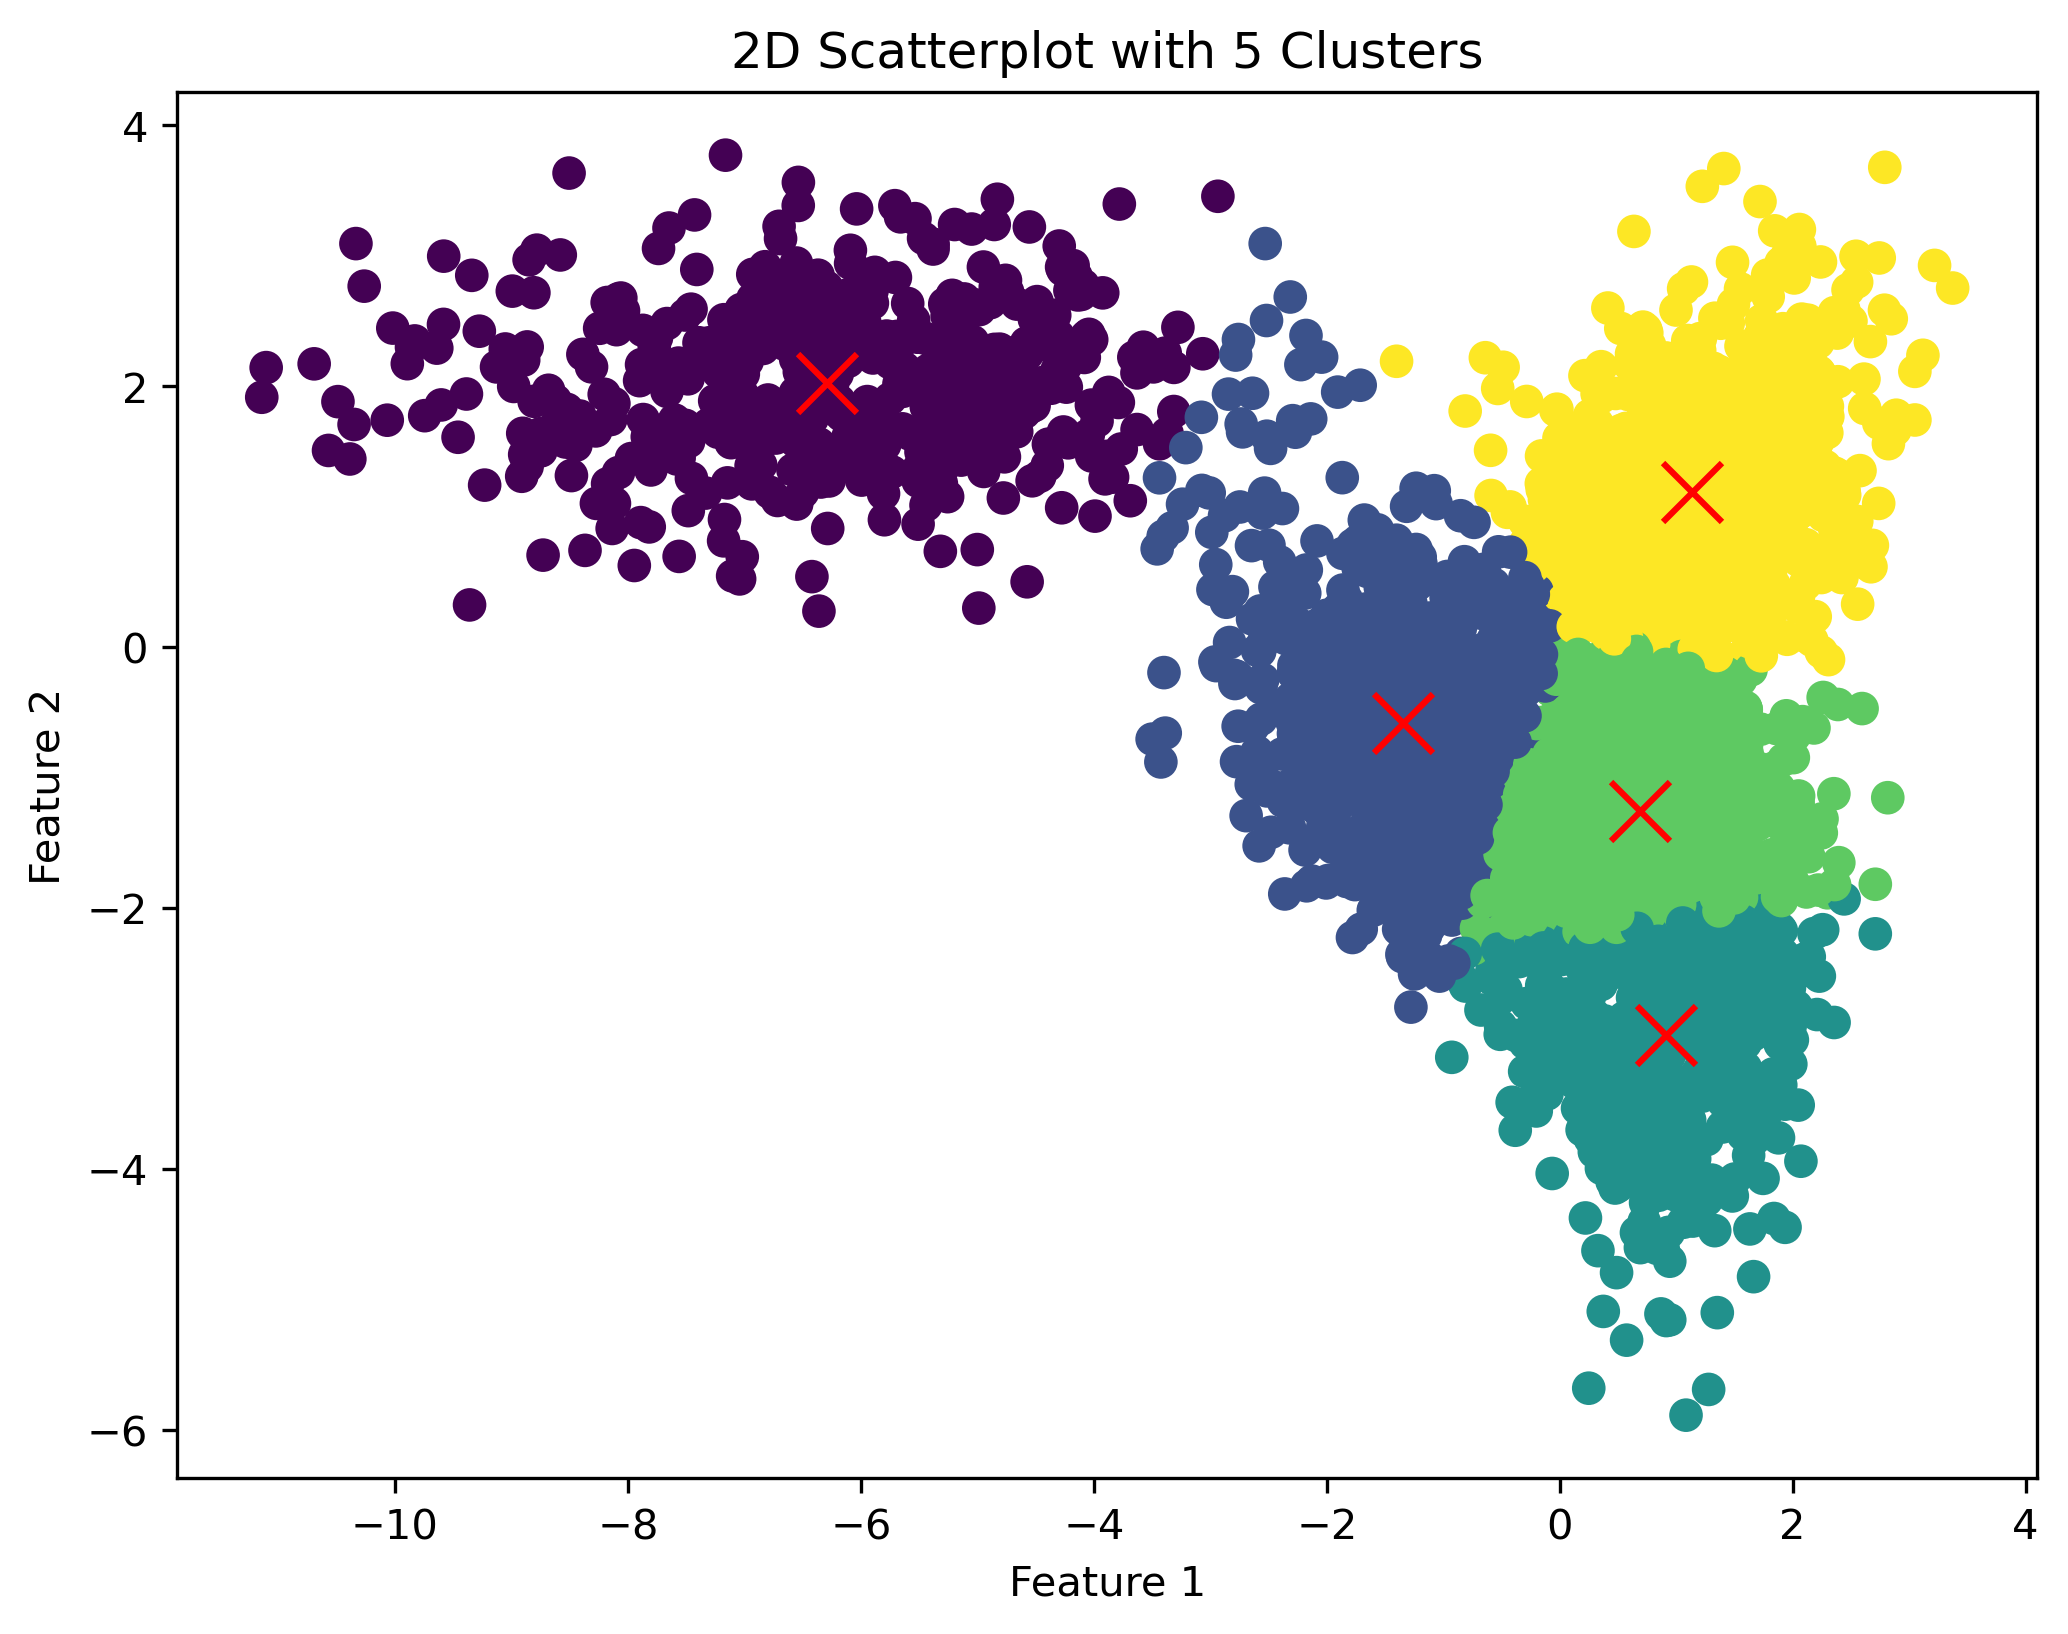
\includegraphics[width=\textwidth]{figures/random_2d_scatter_k5_d0.png}
        \caption{$k=5$ (Dataset 1)}
        \label{fig:2d_k5}
    \end{subfigure}
    \begin{subfigure}[b]{0.45\textwidth}
        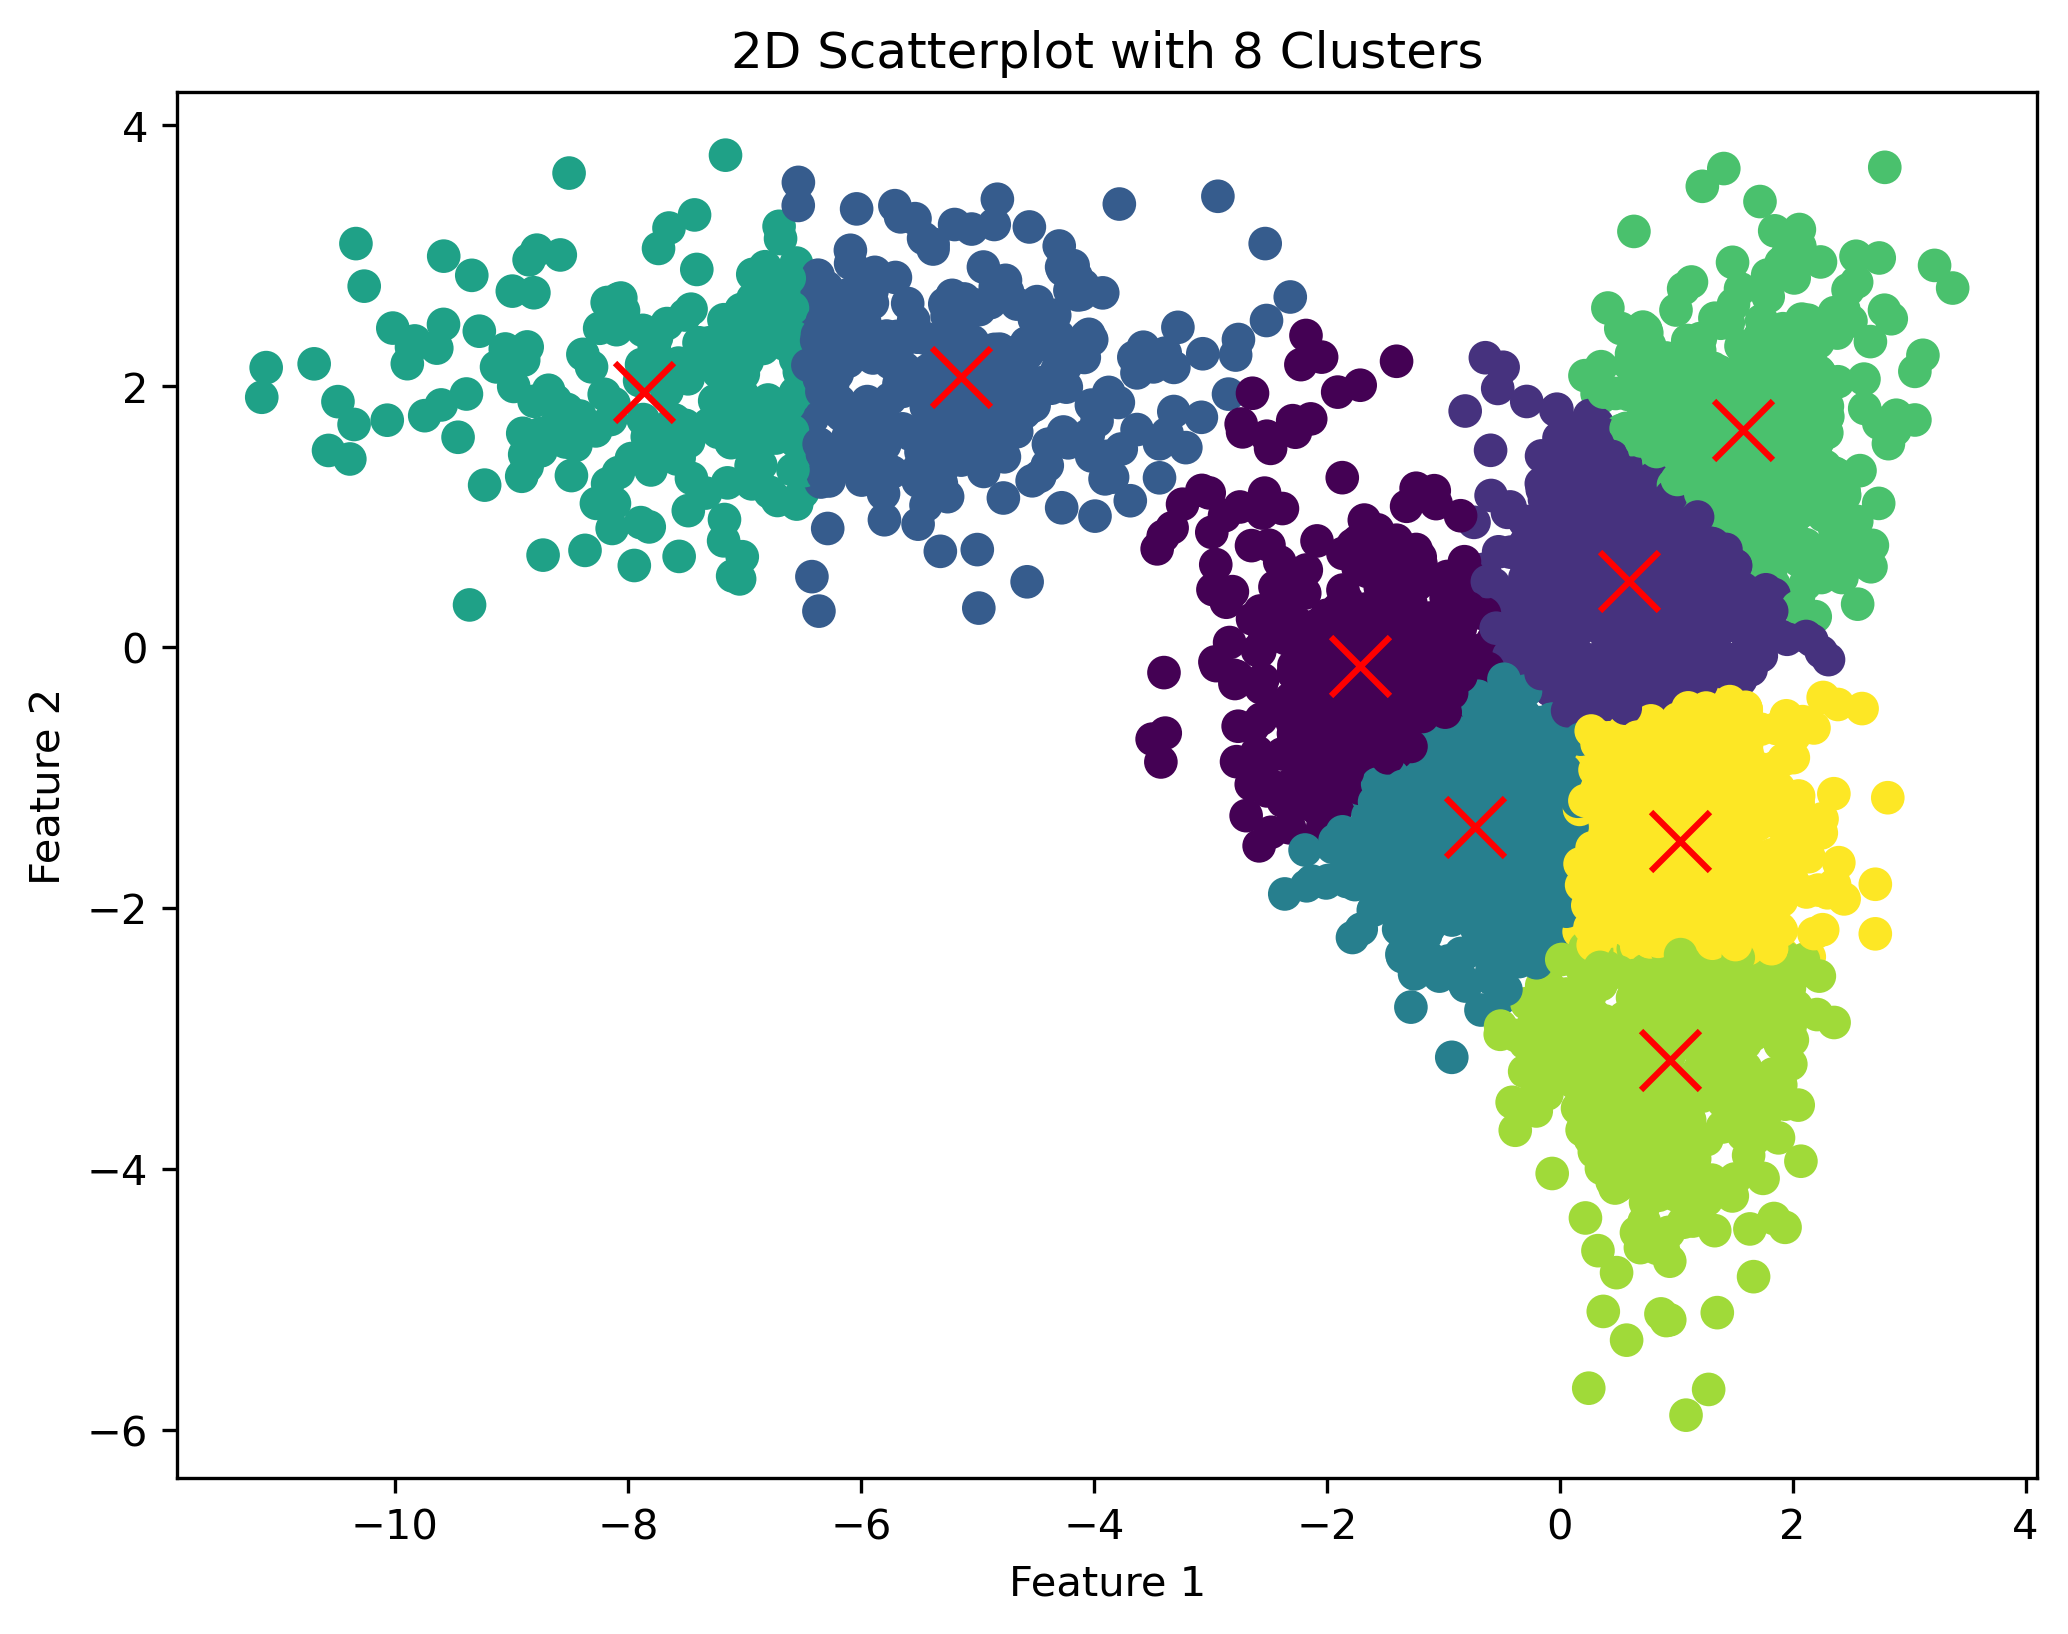
\includegraphics[width=\textwidth]{figures/random_2d_scatter_k8_d0.png}
        \caption{$k=8$ (Dataset 1)}
        \label{fig:2d_k8}
    \end{subfigure}
    \begin{subfigure}[b]{0.45\textwidth}
        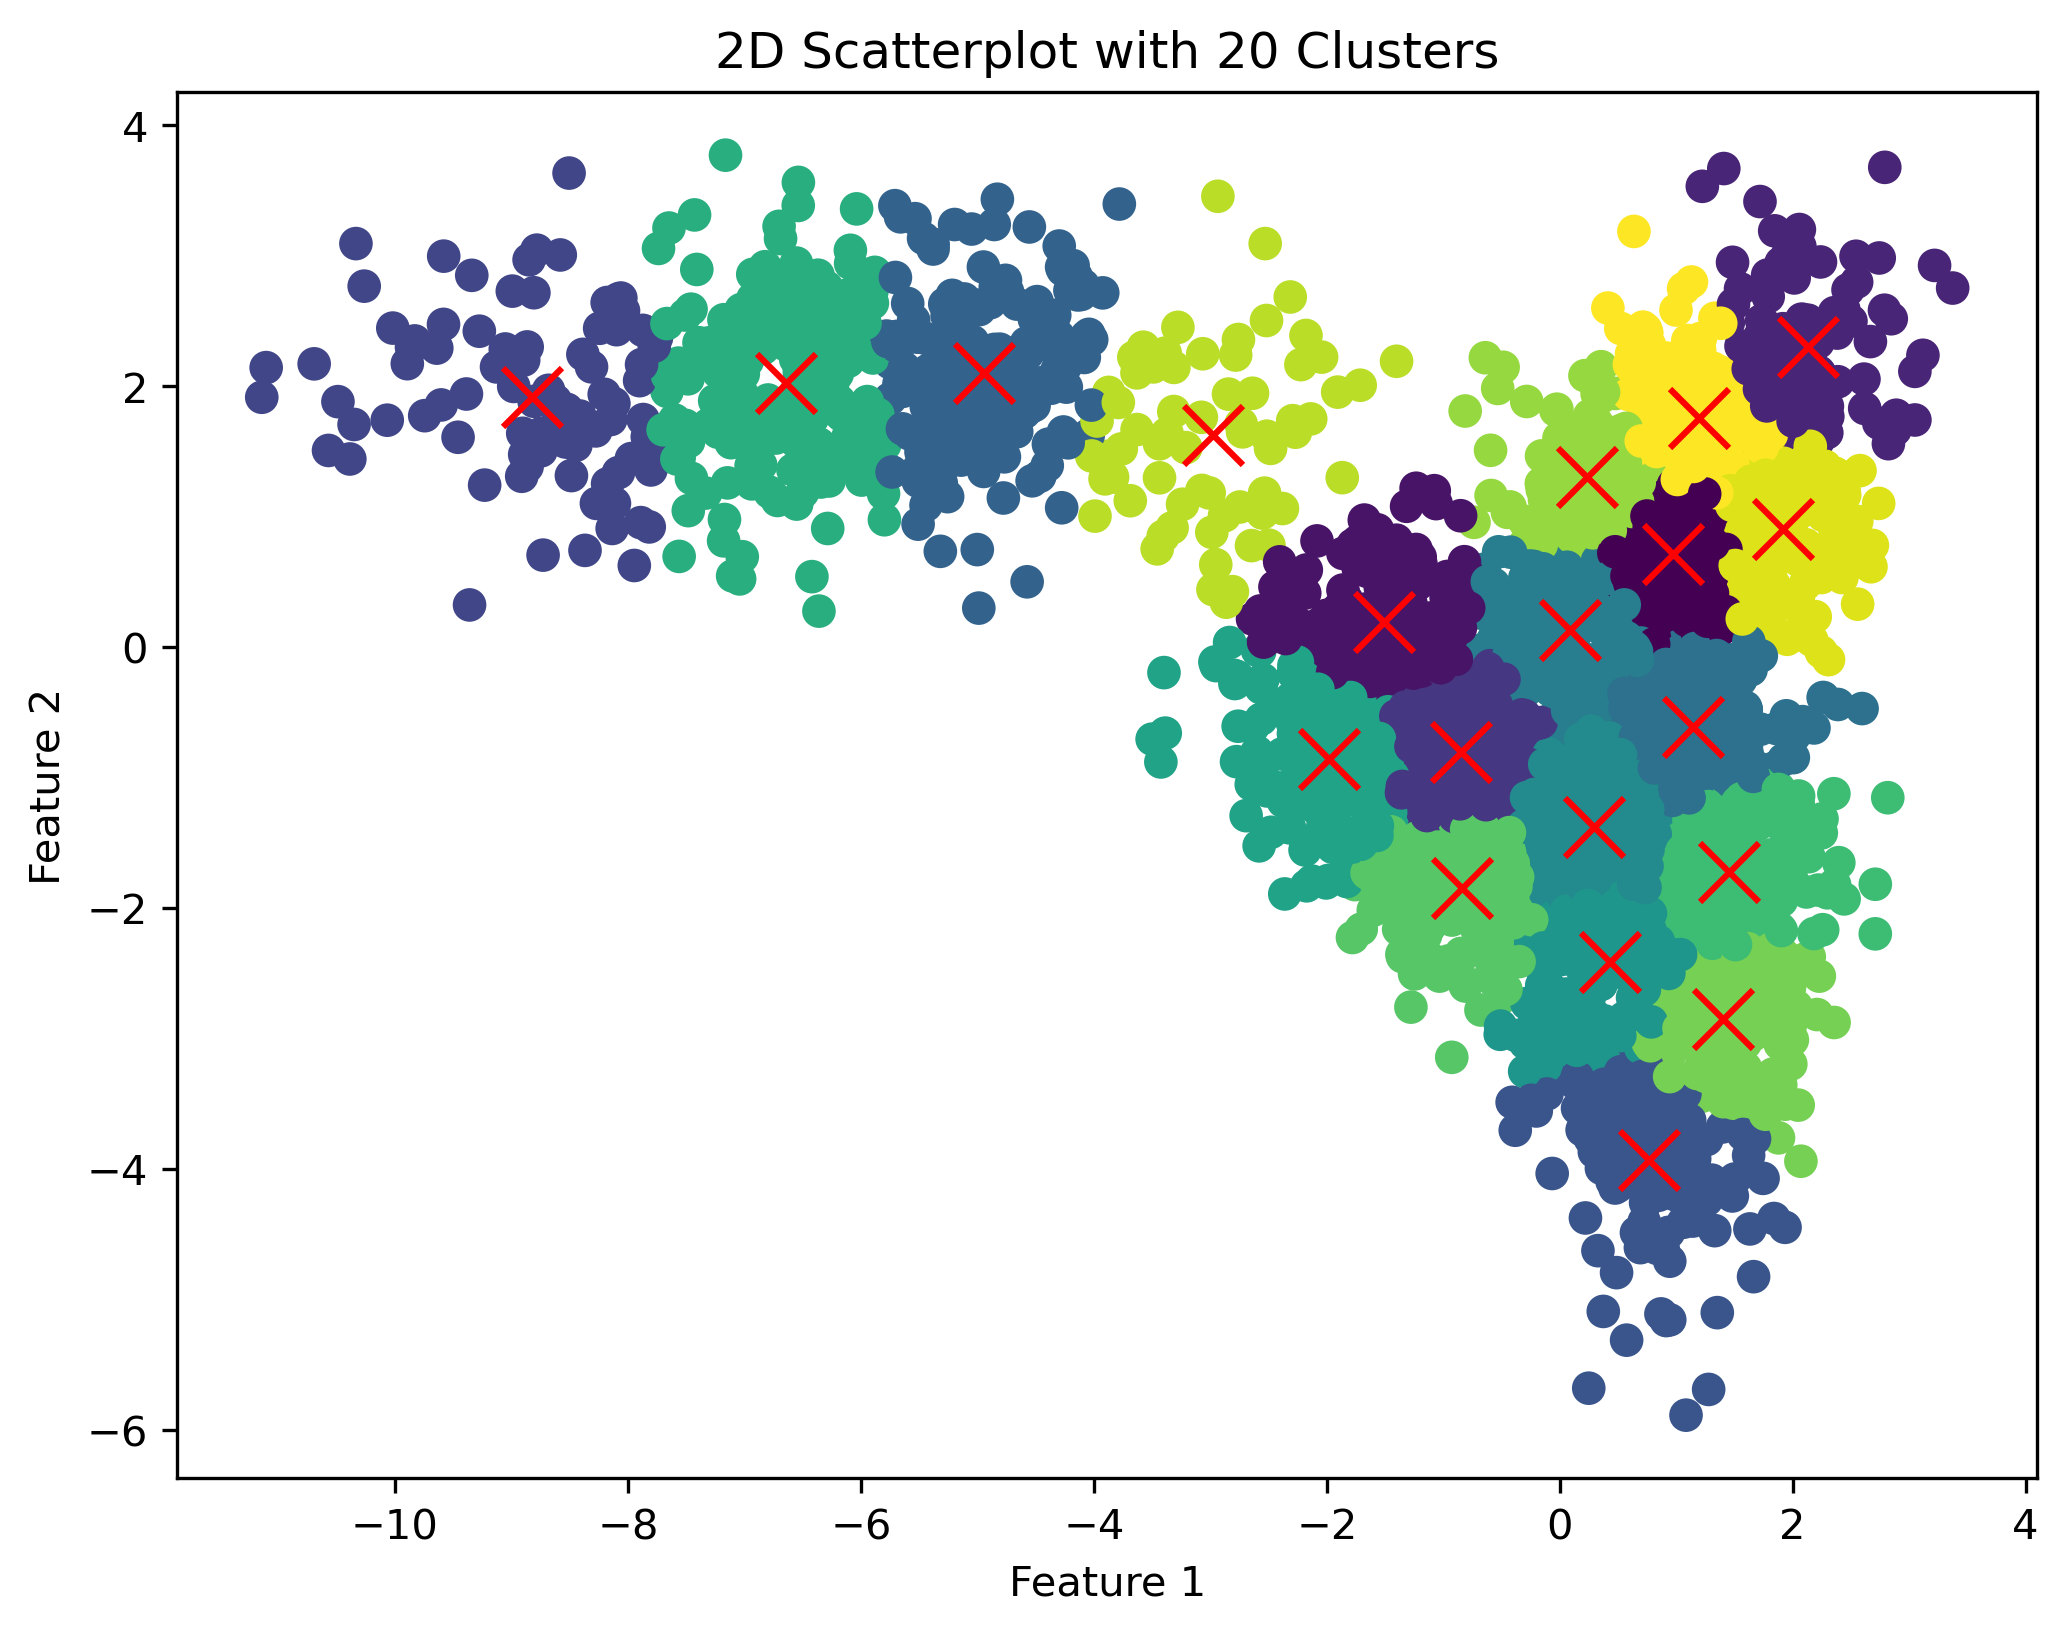
\includegraphics[width=\textwidth]{figures/random_2d_scatter_k20_d0.png}
        \caption{$k=20$ (Dataset 1)}
        \label{fig:2d_k20}
    \end{subfigure}
    \caption{Scatterplots for k-means clustering with random initialization on Dataset 1 (2D)}
    \label{fig:2d_scatterplots}
\end{figure}

\begin{figure}[h]
    \centering
    \begin{subfigure}[b]{0.45\textwidth}
        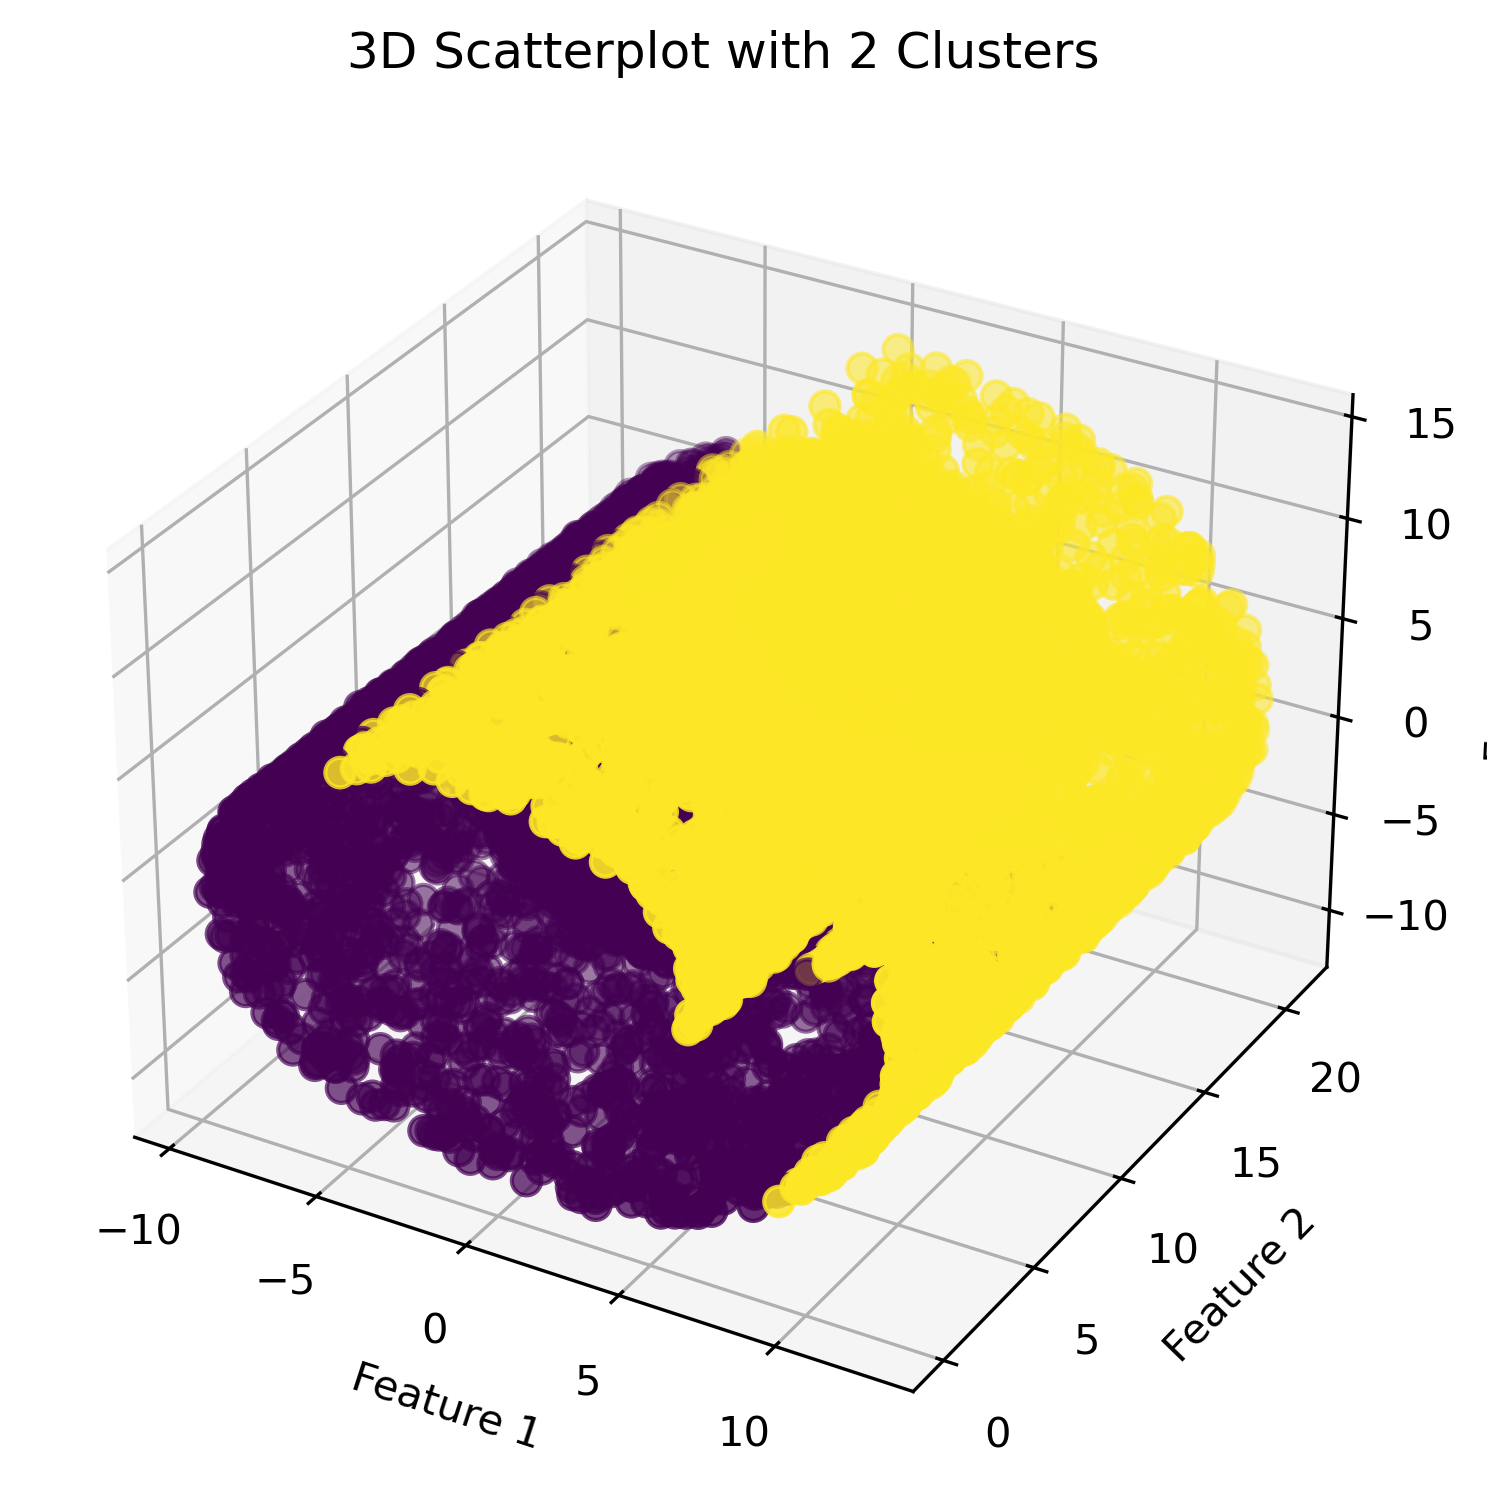
\includegraphics[width=\textwidth]{figures/3d_scatter_k2_d1.png}
        \caption{$k=2$ (Dataset 2)}
        \label{fig:3d_k2}
    \end{subfigure}
    \begin{subfigure}[b]{0.45\textwidth}
        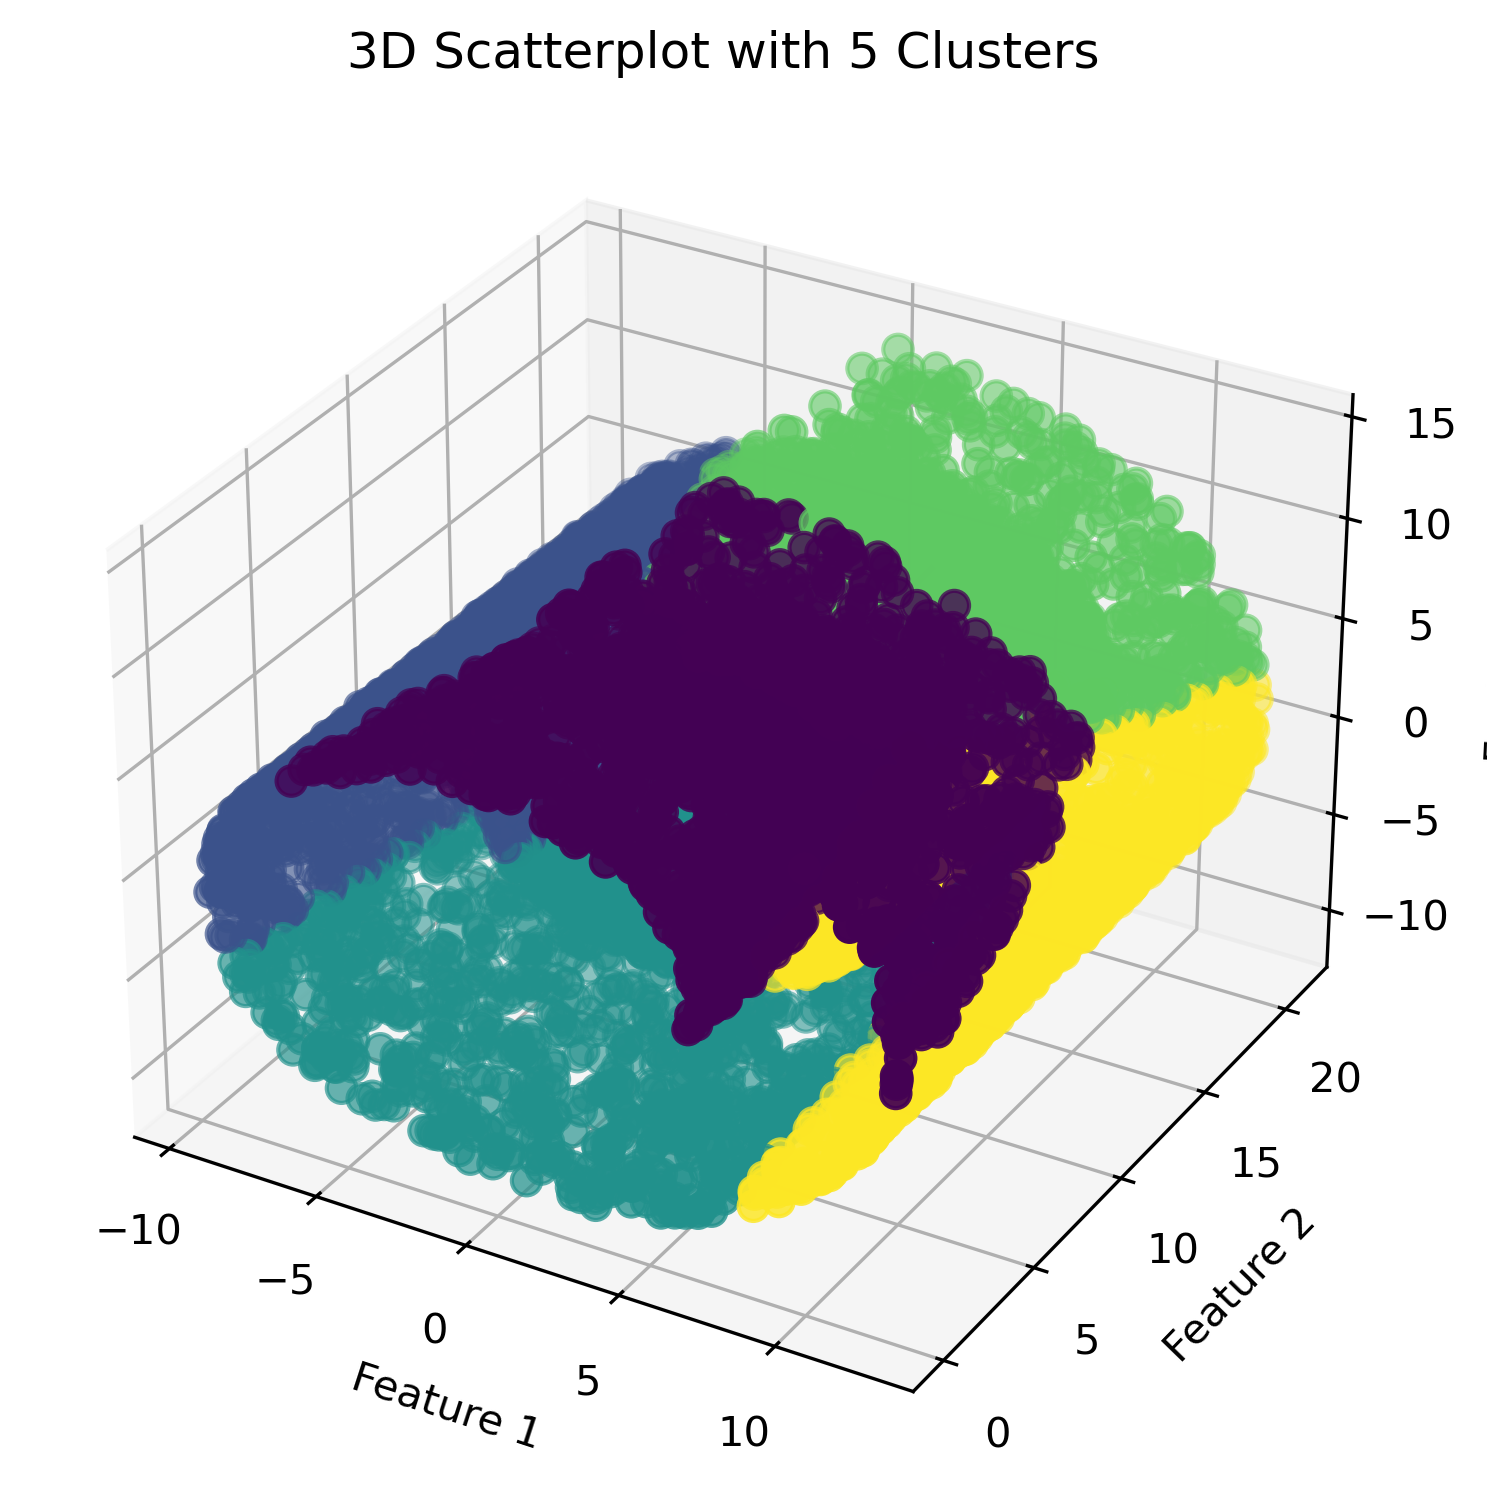
\includegraphics[width=\textwidth]{figures/3d_scatter_k5_d1.png}
        \caption{$k=5$ (Dataset 2)}
        \label{fig:3d_k5}
    \end{subfigure}
    \begin{subfigure}[b]{0.45\textwidth}
        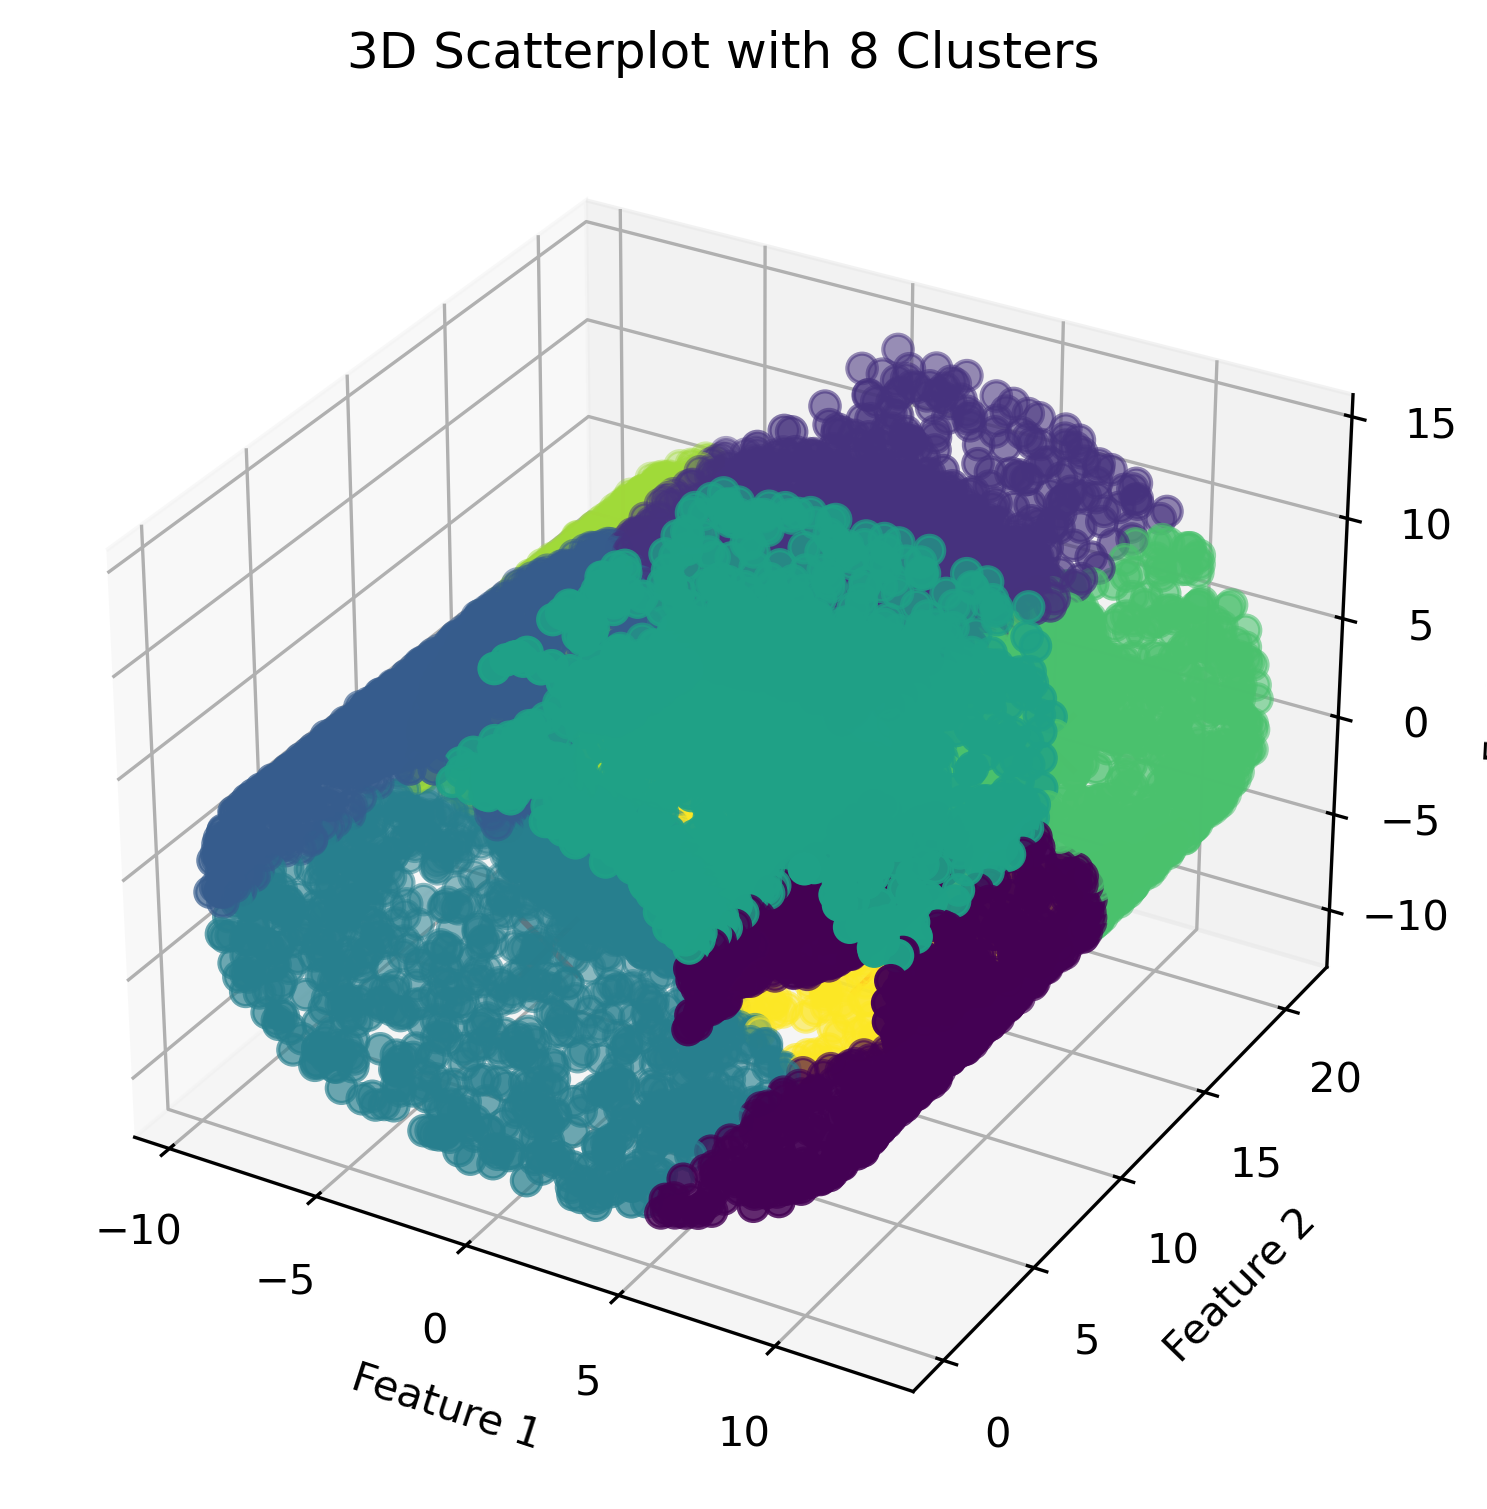
\includegraphics[width=\textwidth]{figures/3d_scatter_k8_d1.png}
        \caption{$k=8$ (Dataset 2)}
        \label{fig:3d_k8}
    \end{subfigure}
    \begin{subfigure}[b]{0.45\textwidth}
        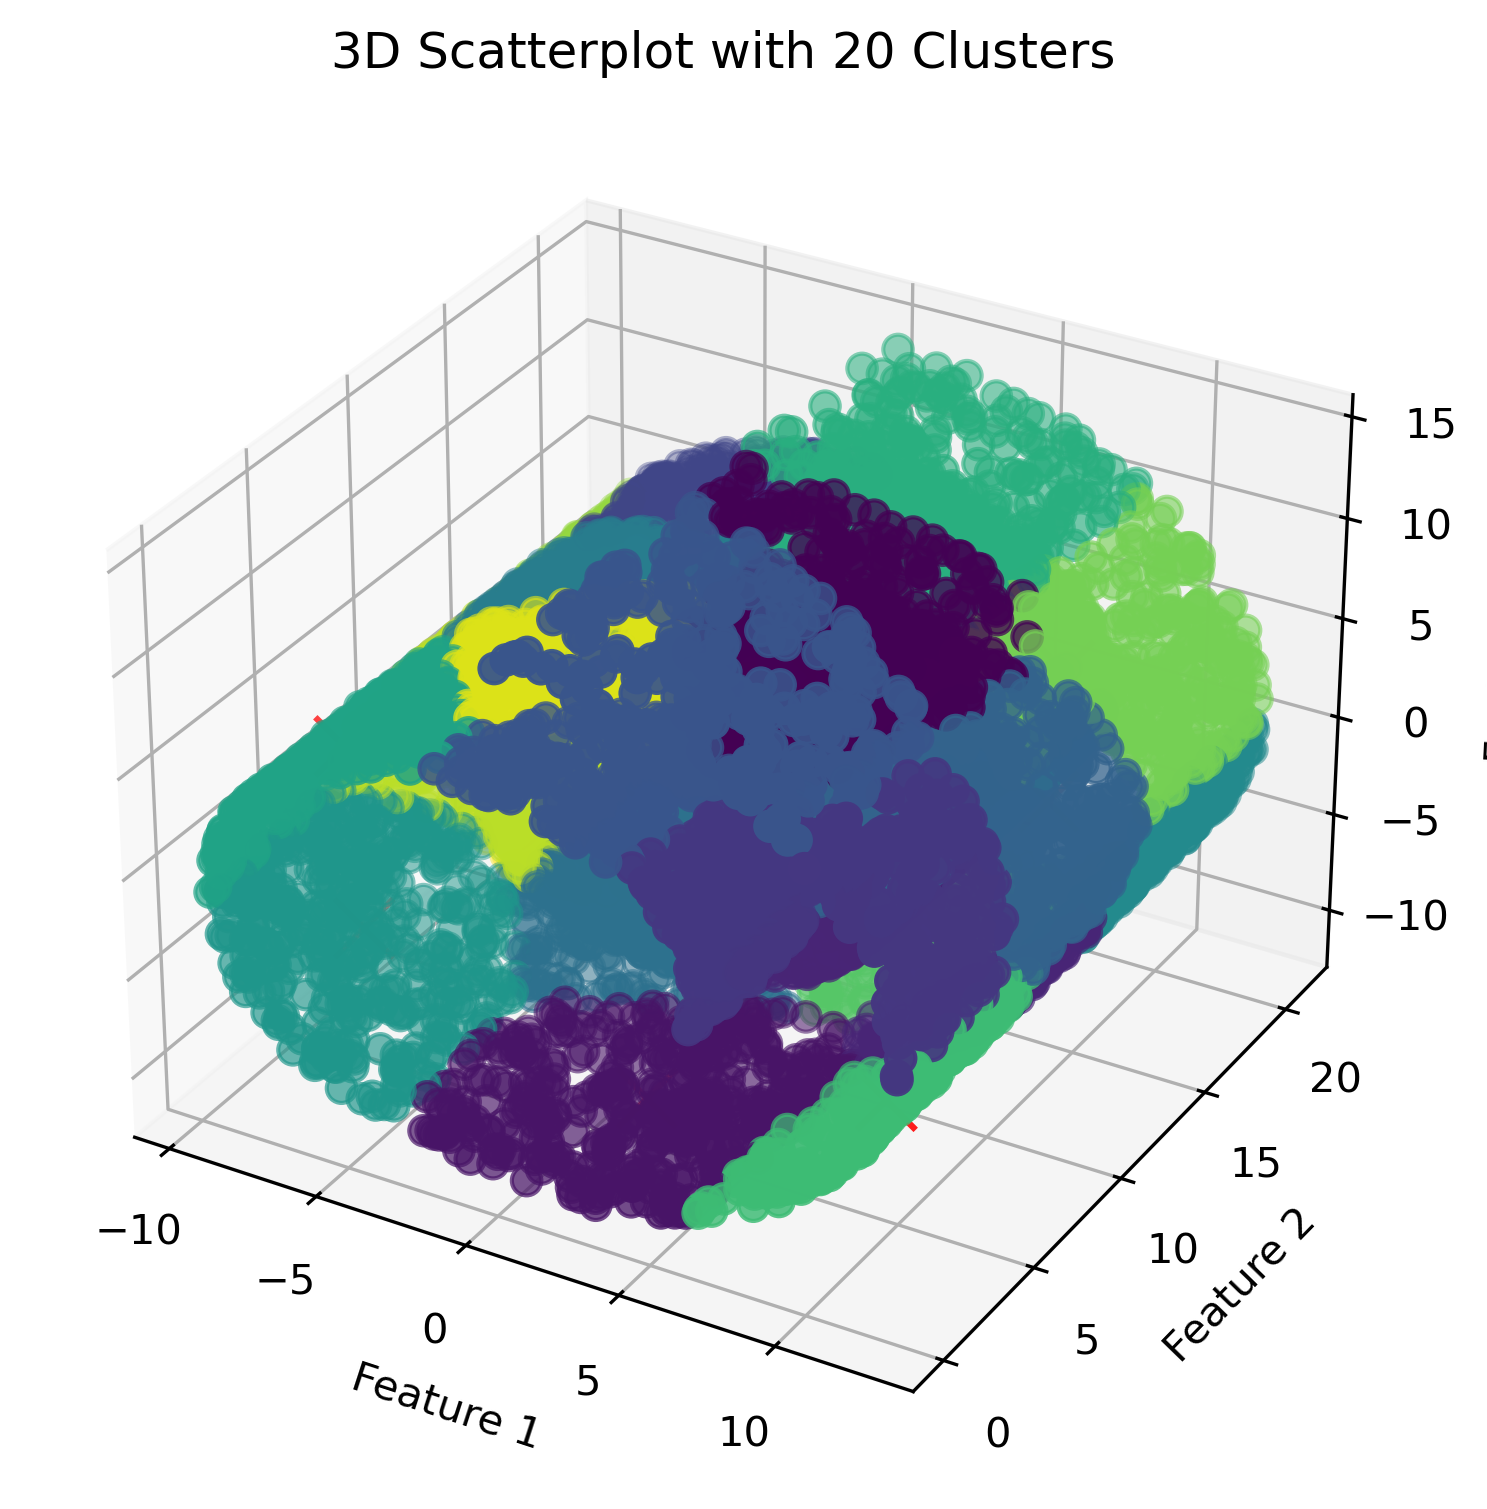
\includegraphics[width=\textwidth]{figures/3d_scatter_k20_d1.png}
        \caption{$k=20$ (Dataset 2)}
        \label{fig:3d_k20}
    \end{subfigure}
    \caption{Scatterplots for k-means clustering on Dataset 2 (3D)}
    \label{fig:3d_scatterplots}
\end{figure}

\begin{figure}[h]
    \centering
    \begin{subfigure}[b]{0.45\textwidth}
        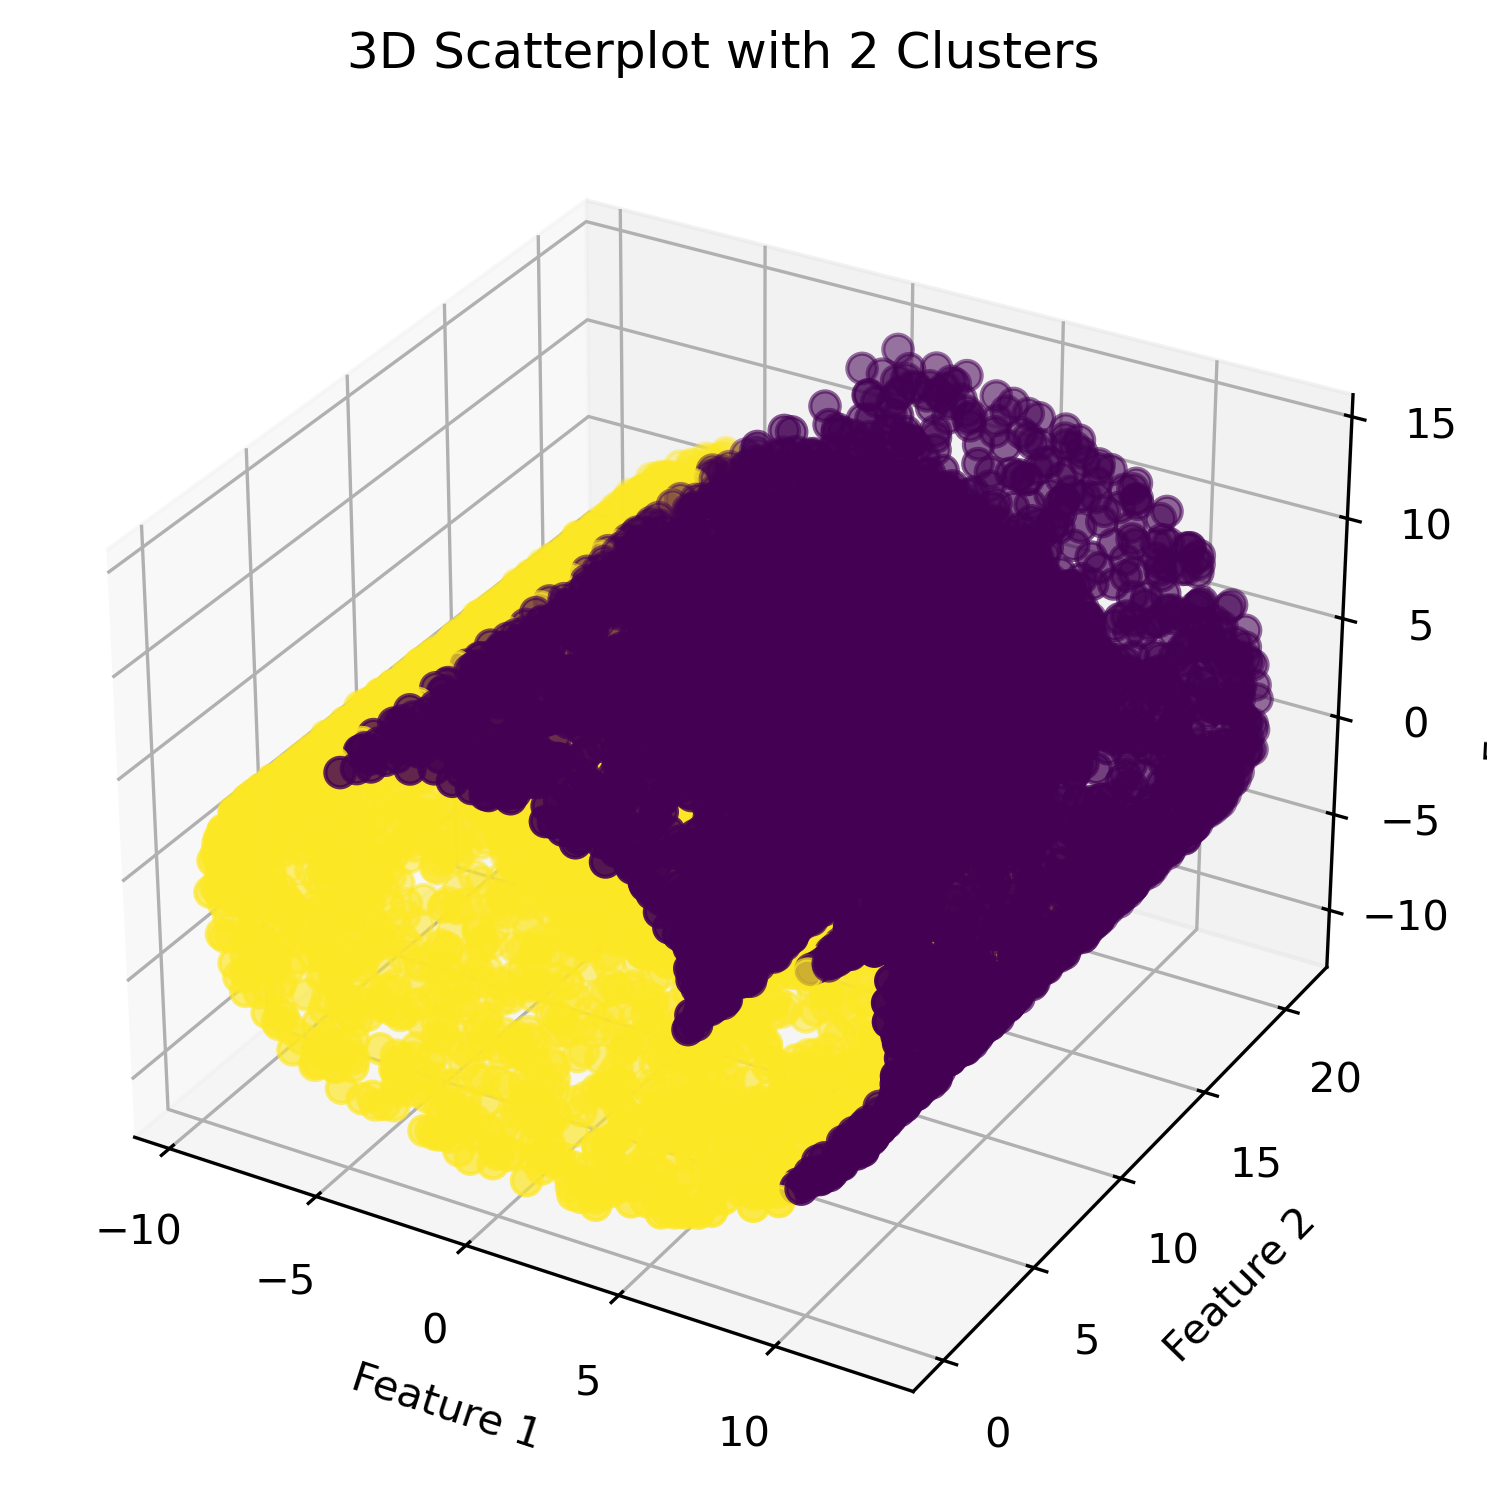
\includegraphics[width=\textwidth]{figures/random_3d_scatter_k2_d1.png}
        \caption{$k=2$ (Dataset 2)}
        \label{fig:3d_k2}
    \end{subfigure}
    \begin{subfigure}[b]{0.45\textwidth}
        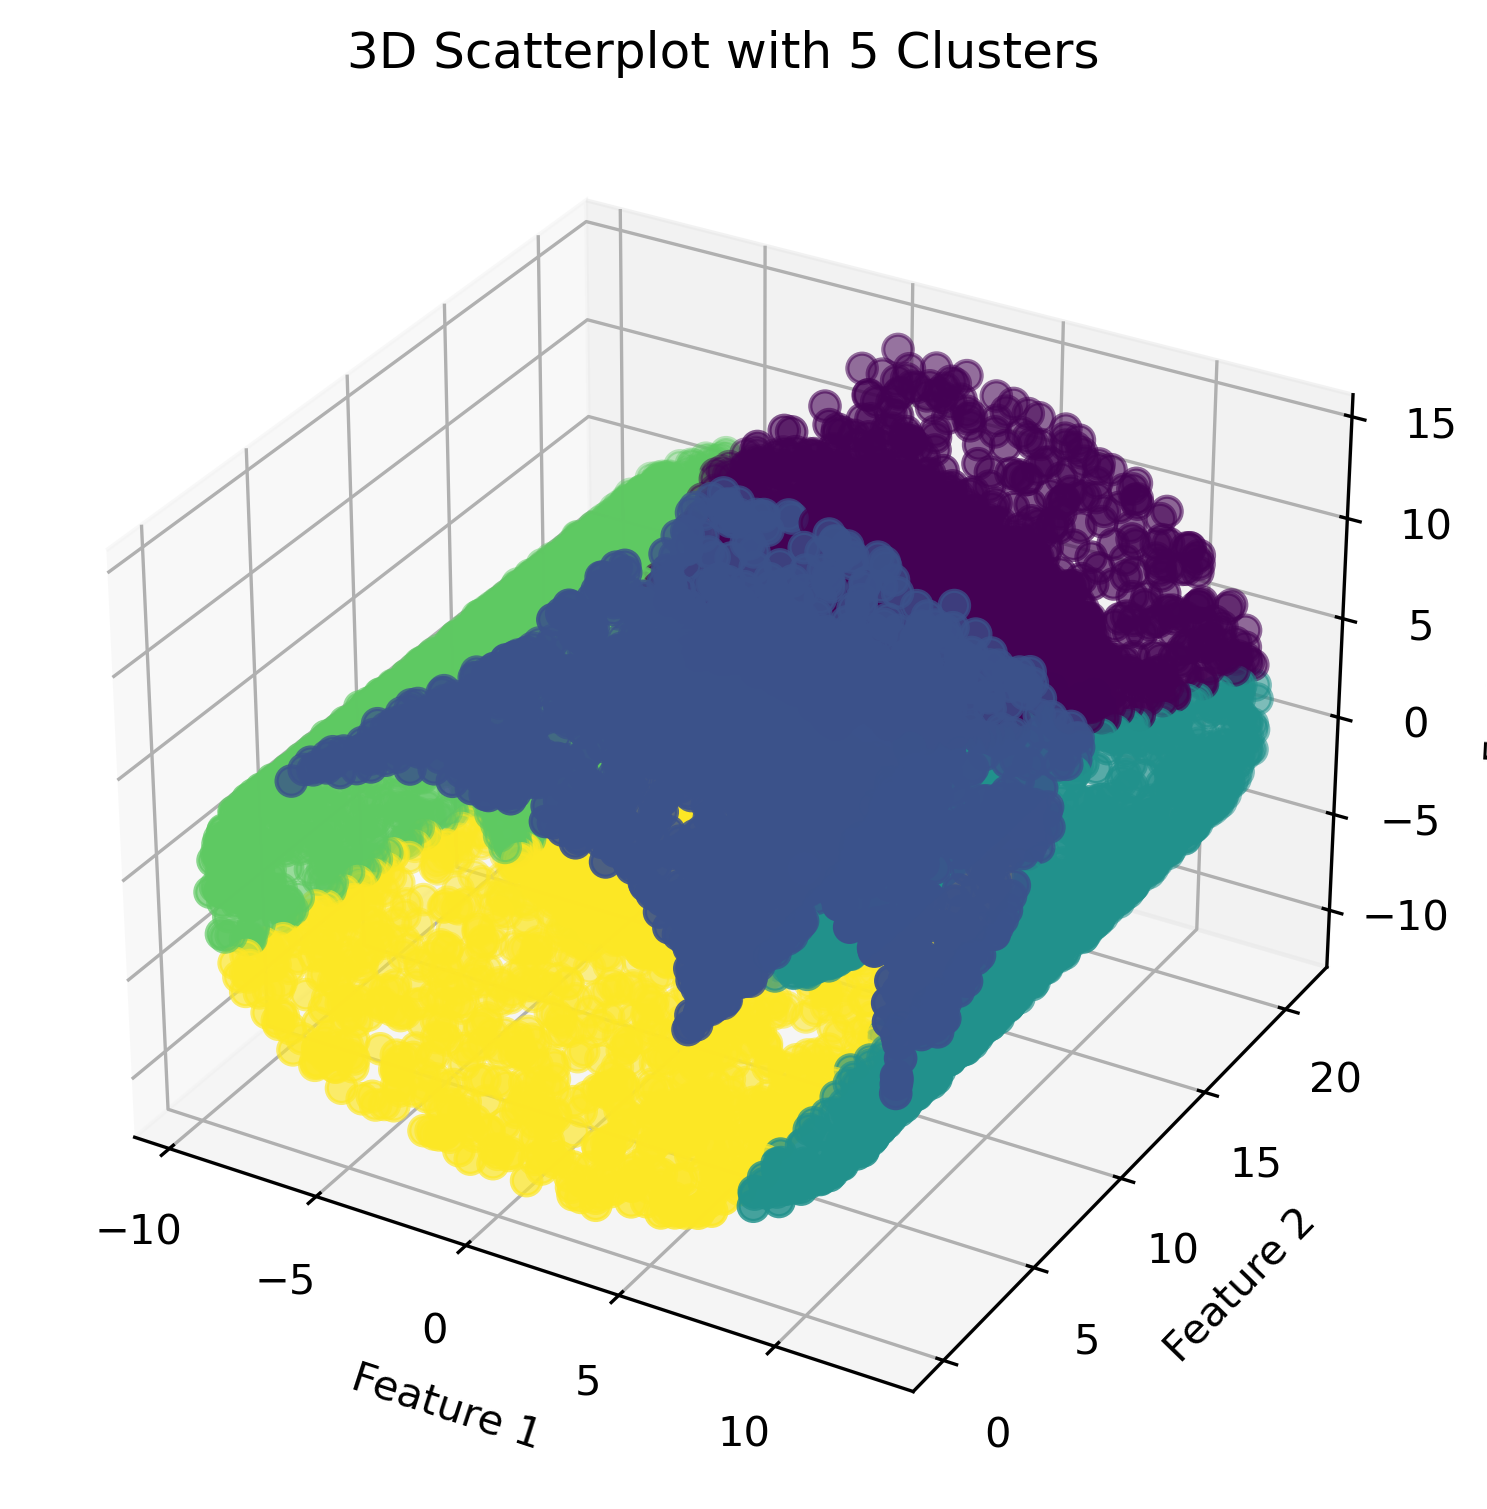
\includegraphics[width=\textwidth]{figures/random_3d_scatter_k5_d1.png}
        \caption{$k=5$ (Dataset 2)}
        \label{fig:3d_k5}
    \end{subfigure}
    \begin{subfigure}[b]{0.45\textwidth}
        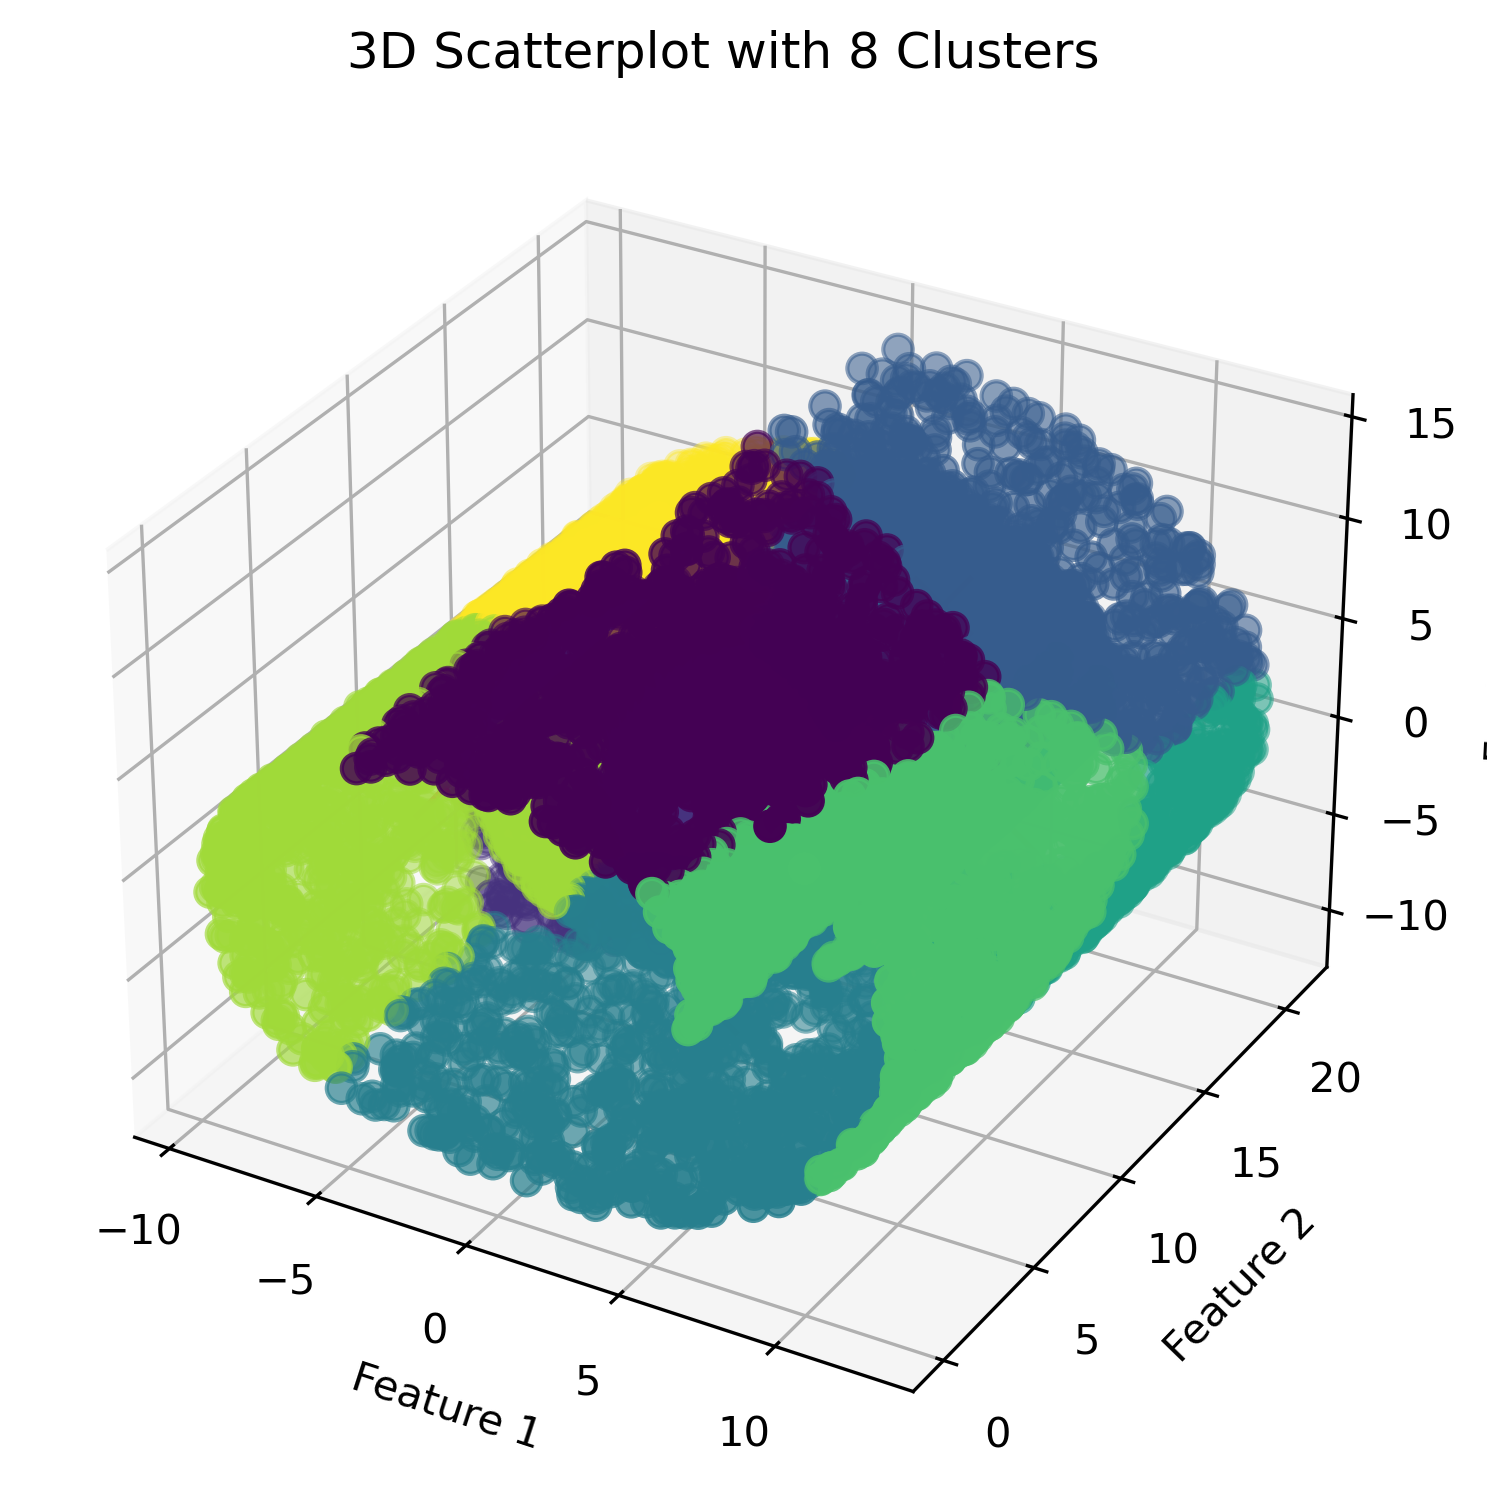
\includegraphics[width=\textwidth]{figures/random_3d_scatter_k8_d1.png}
        \caption{$k=8$ (Dataset 2)}
        \label{fig:3d_k8}
    \end{subfigure}
    \begin{subfigure}[b]{0.45\textwidth}
        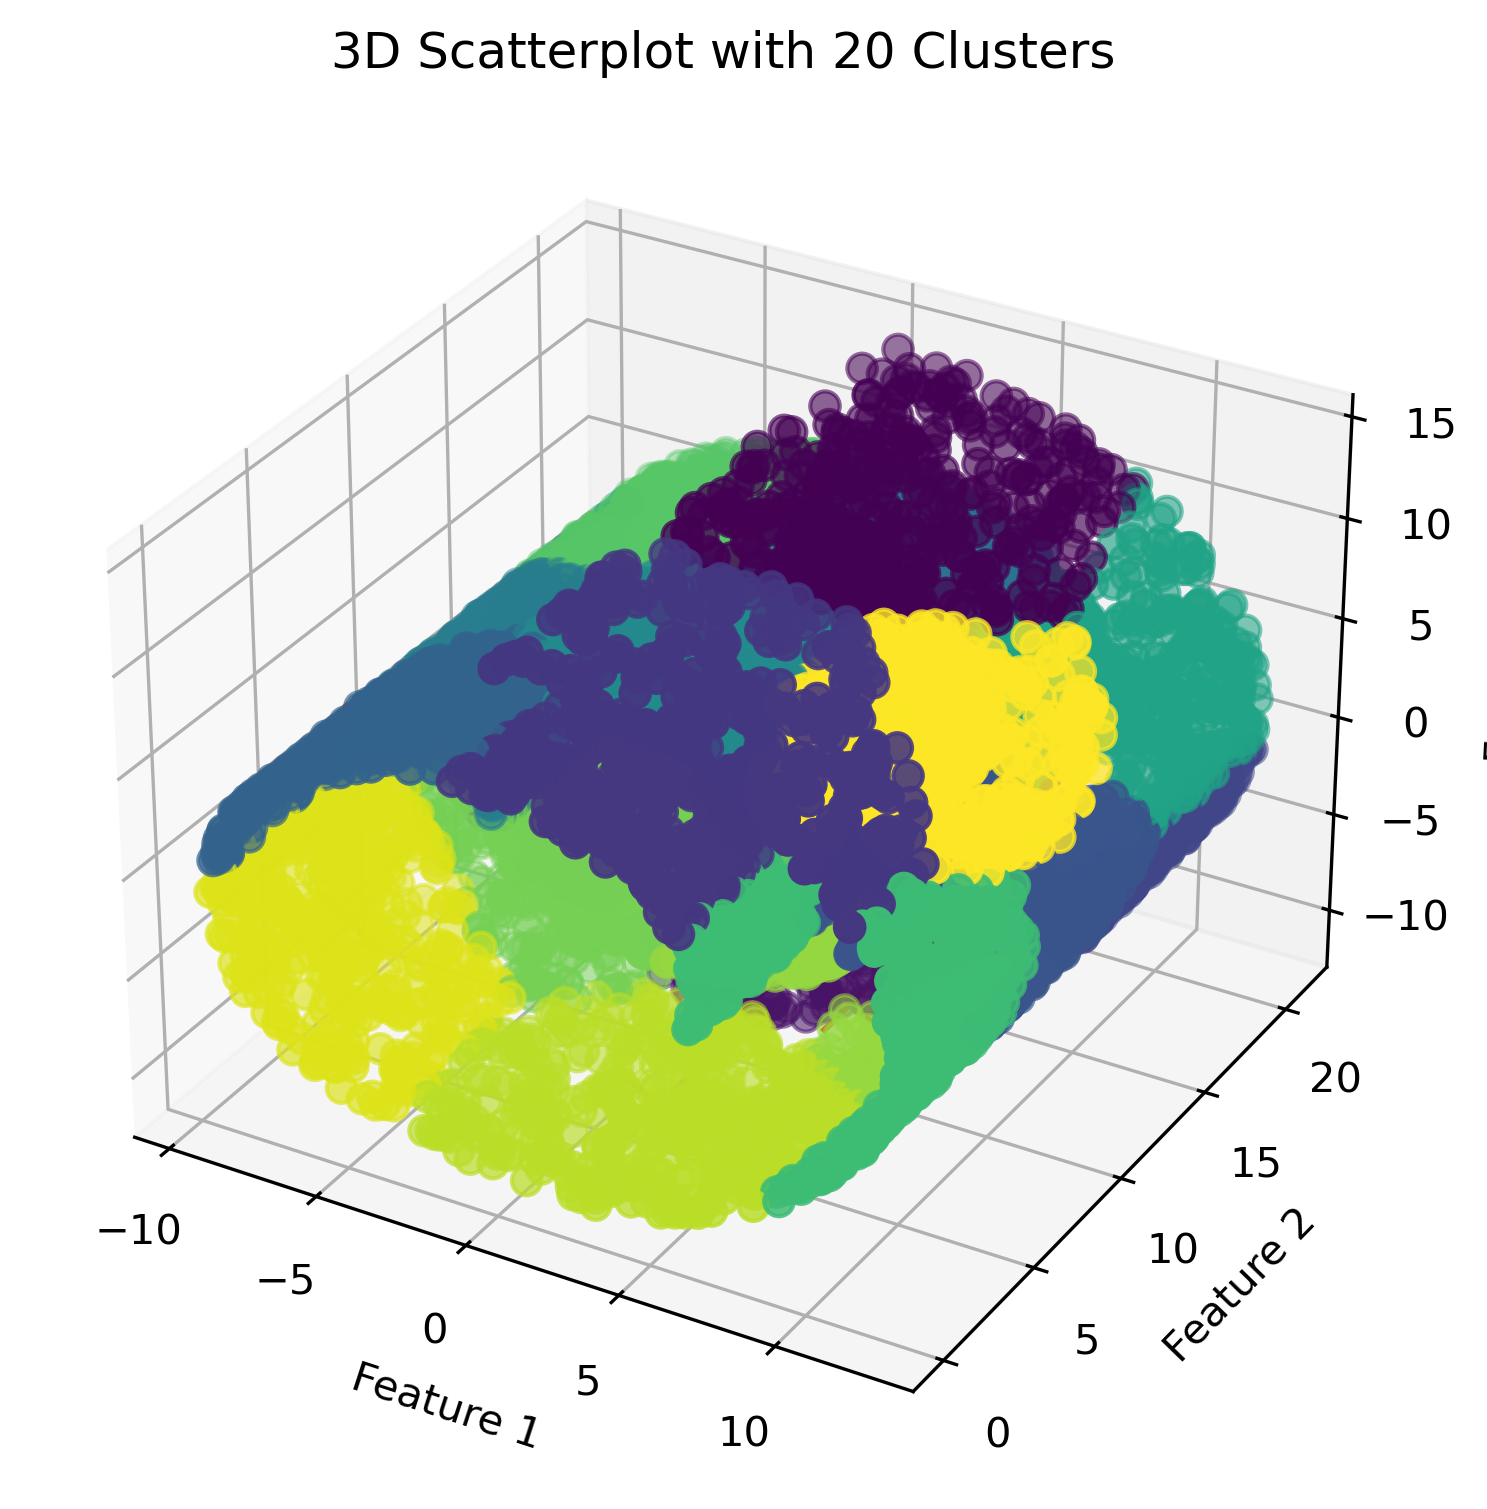
\includegraphics[width=\textwidth]{figures/random_3d_scatter_k20_d1.png}
        \caption{$k=20$ (Dataset 2)}
        \label{fig:3d_k20}
    \end{subfigure}
    \caption{Scatterplots for k-means clustering with random initalization on Dataset 2 (3D)}
    \label{fig:3d_scatterplots}
\end{figure}

\subsection{Hierarchical Agglomerative Clustering Results}
Dendrograms were analyzed to determine an appropriate cut-off for clustering.

\begin{figure}[h]
    \centering
    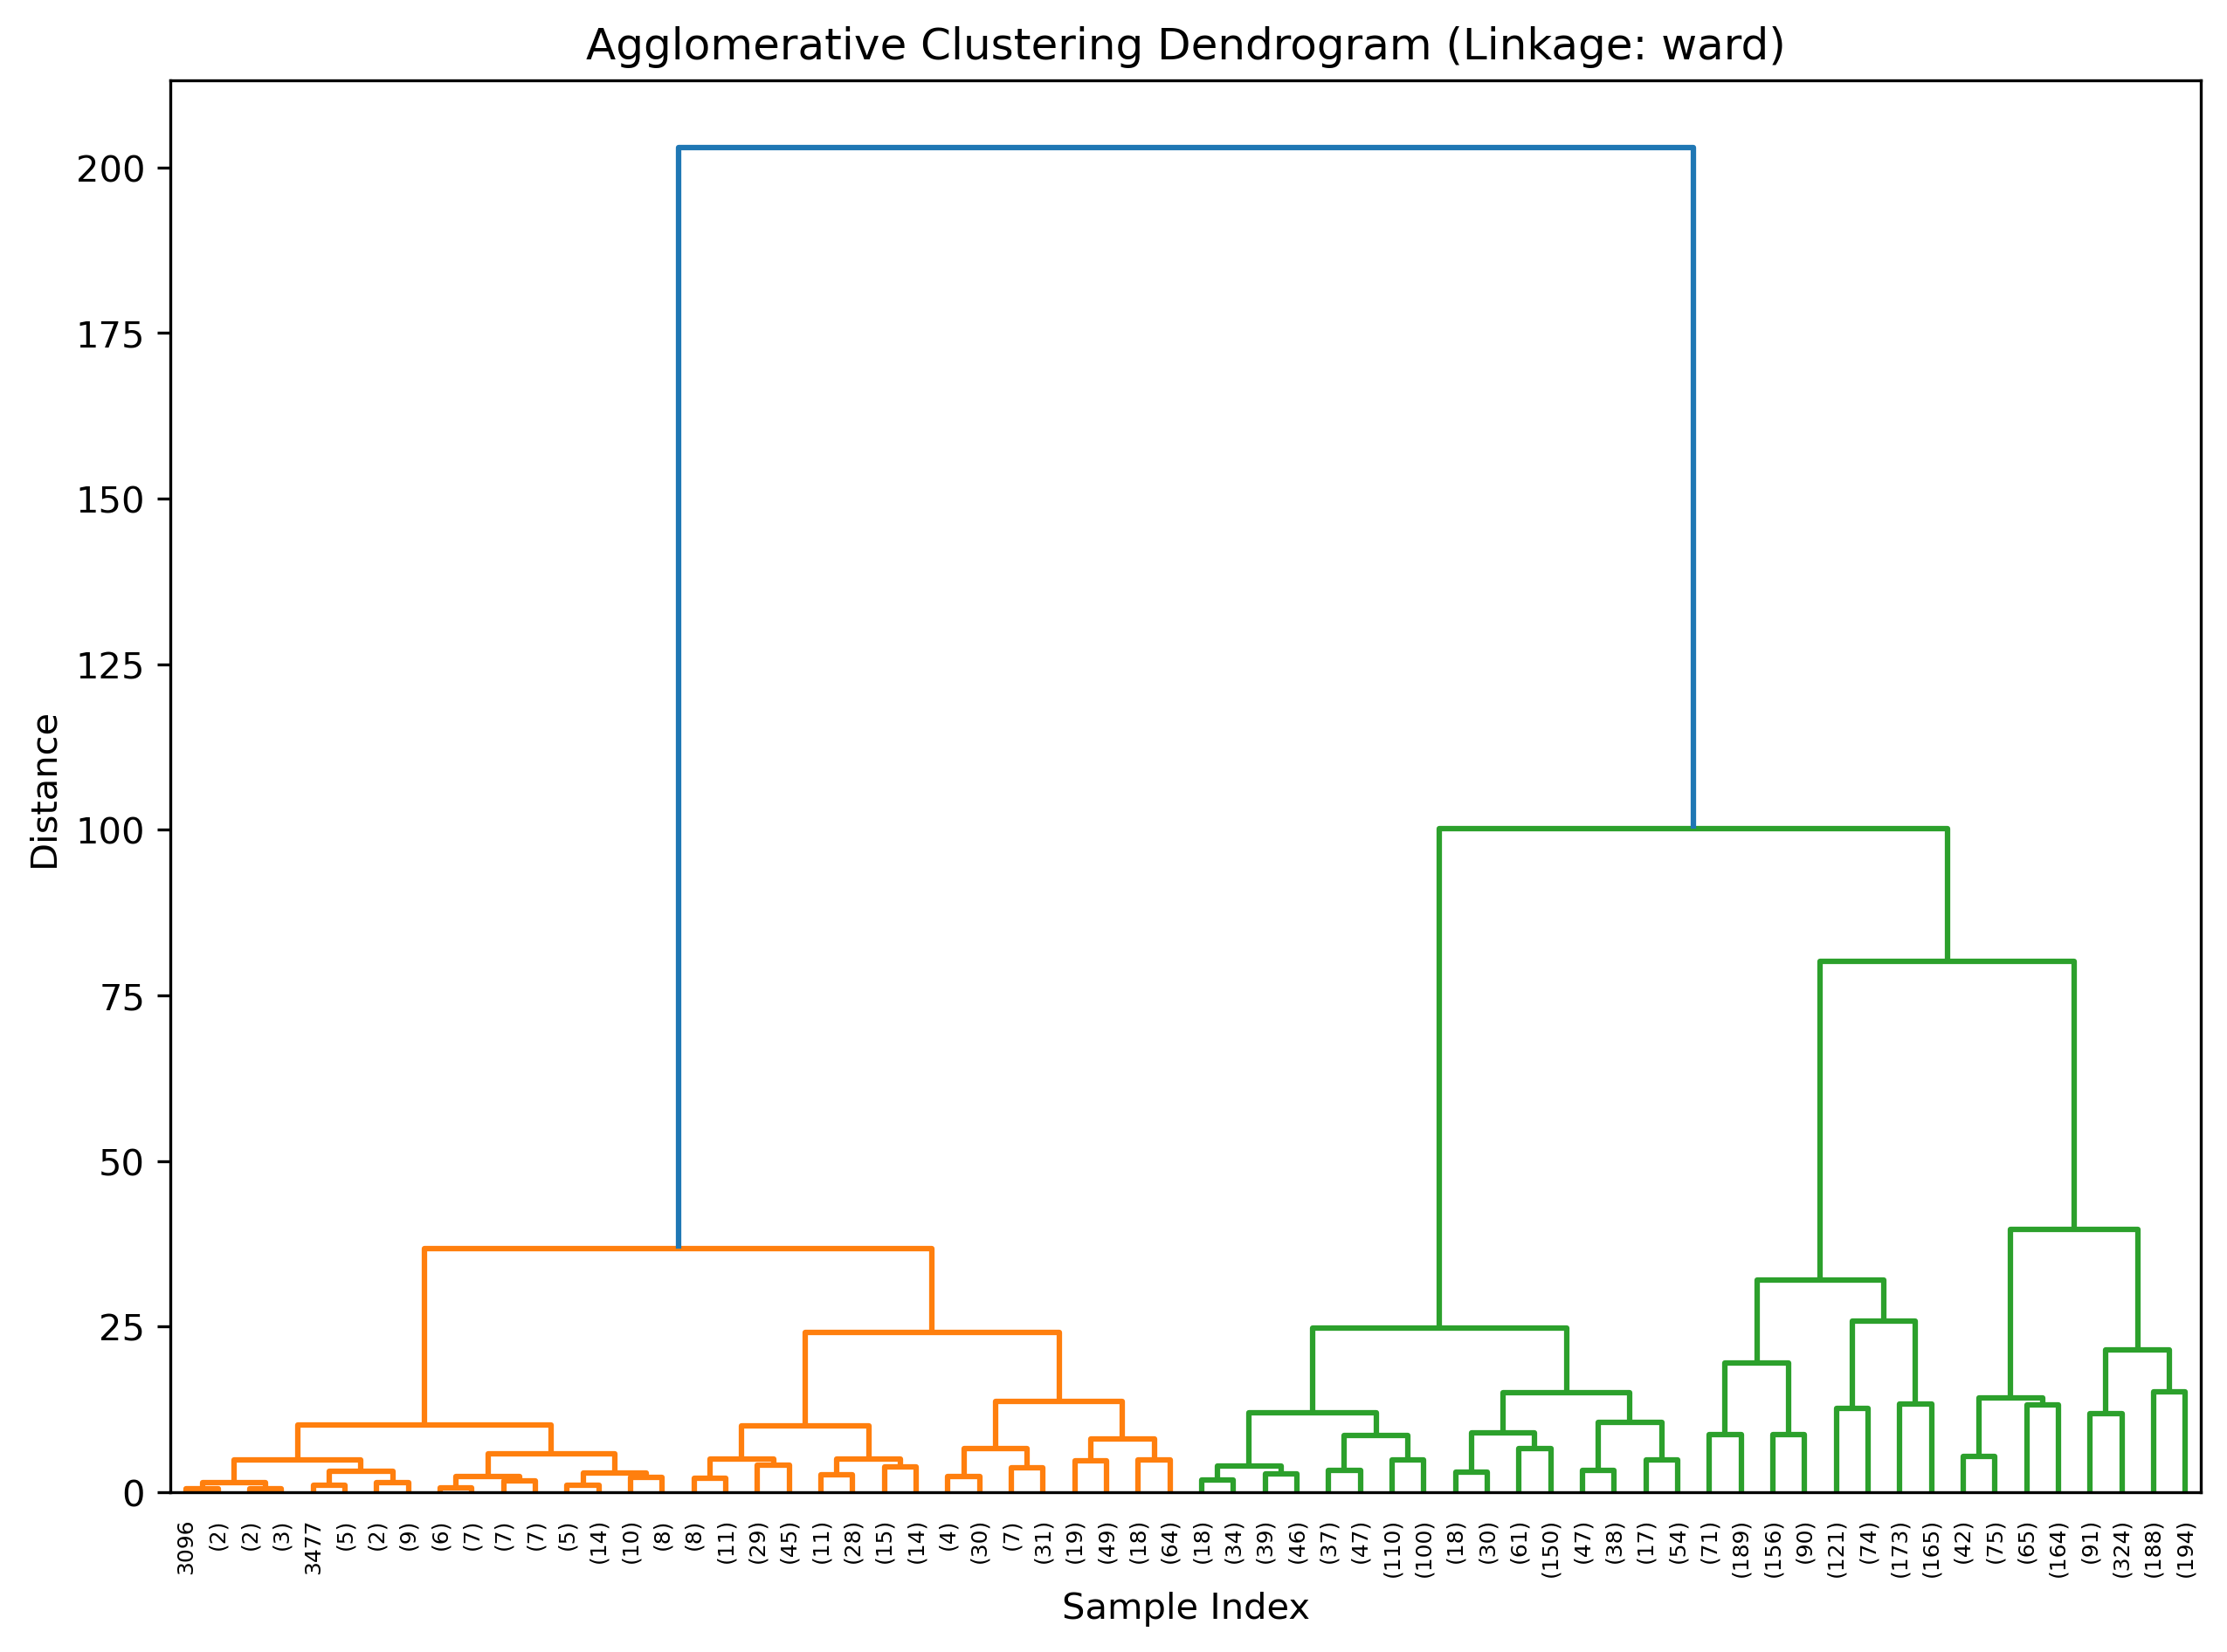
\includegraphics[width=0.7\textwidth]{figures/dendrogram_d0.png} % Replace with actual figure
    \caption{Dendrogram for hierarchical clustering (Dataset 1)}
    \label{fig:dendrogram1}
\end{figure}

\begin{figure}[h]
    \centering
    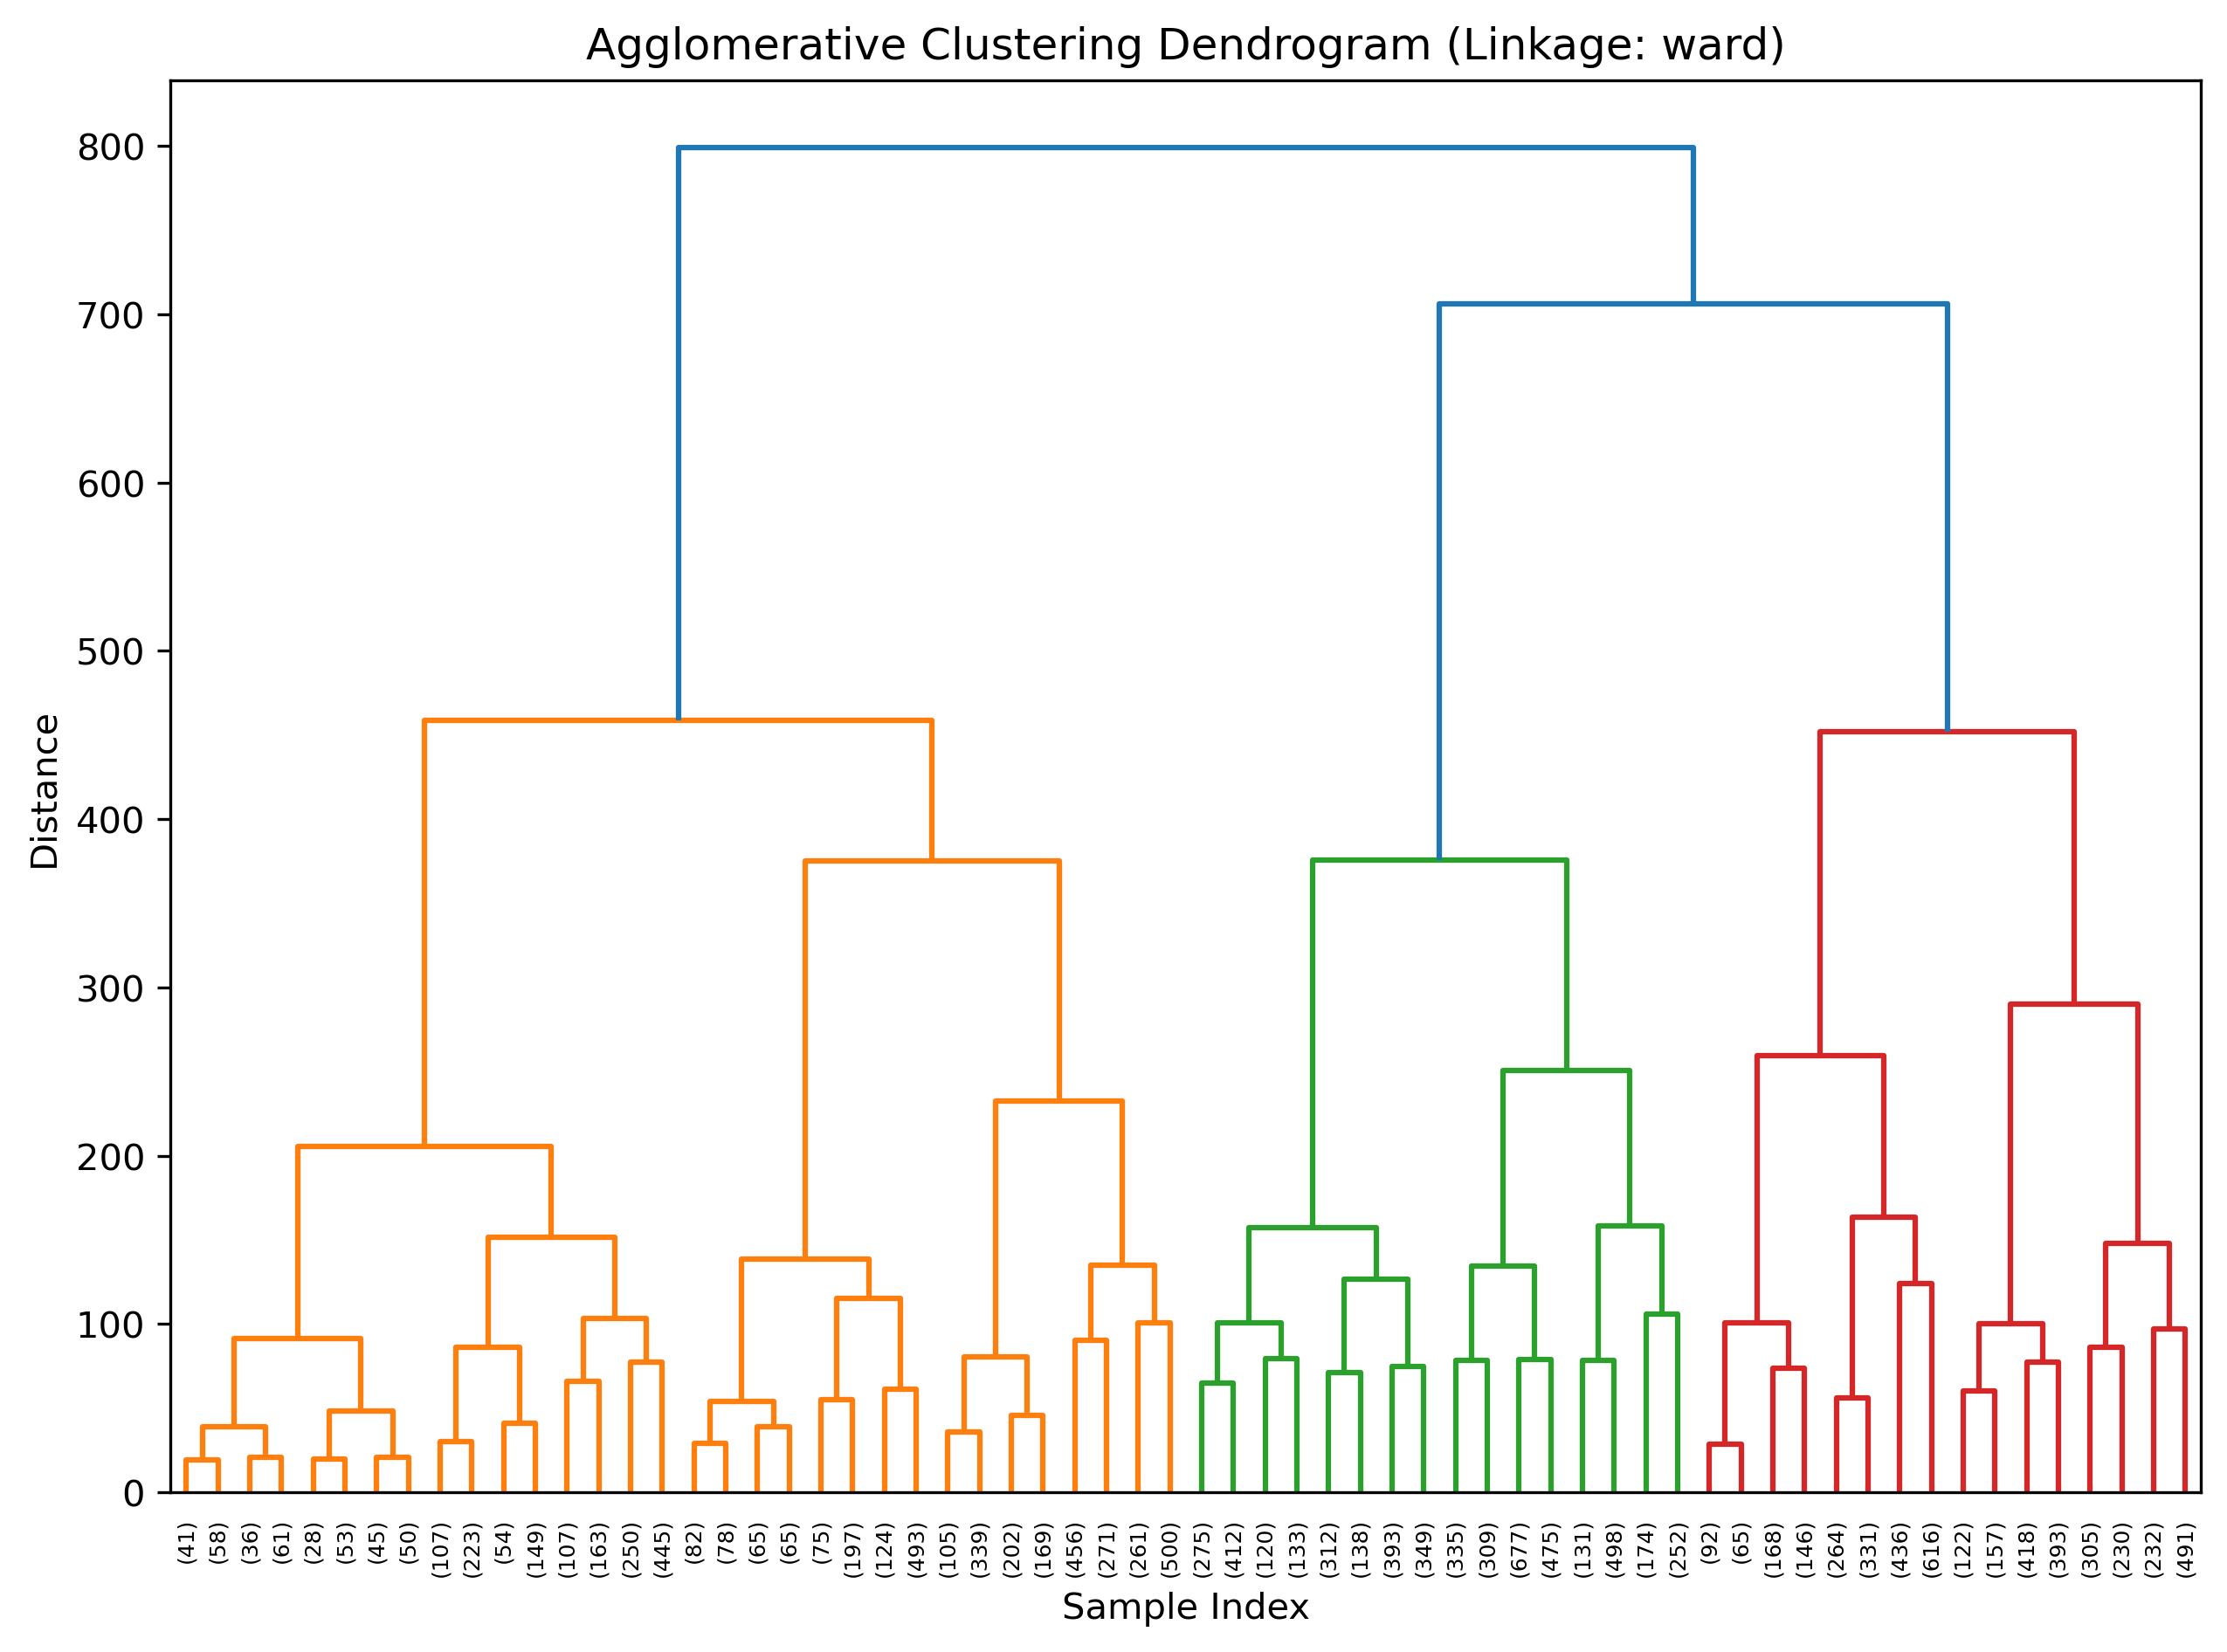
\includegraphics[width=0.7\textwidth]{figures/dendrogram_d1.png} % Replace with actual figure
    \caption{Dendrogram for hierarchical clustering (Dataset 2)}
    \label{fig:dendrogram2}
\end{figure}

\subsection{Scatterplots for Agglomerative Clustering}
The scatterplots for agglomerative clustering are shown below for both datasets.

\begin{figure}[h]
    \centering
    \begin{subfigure}[b]{0.45\textwidth}
        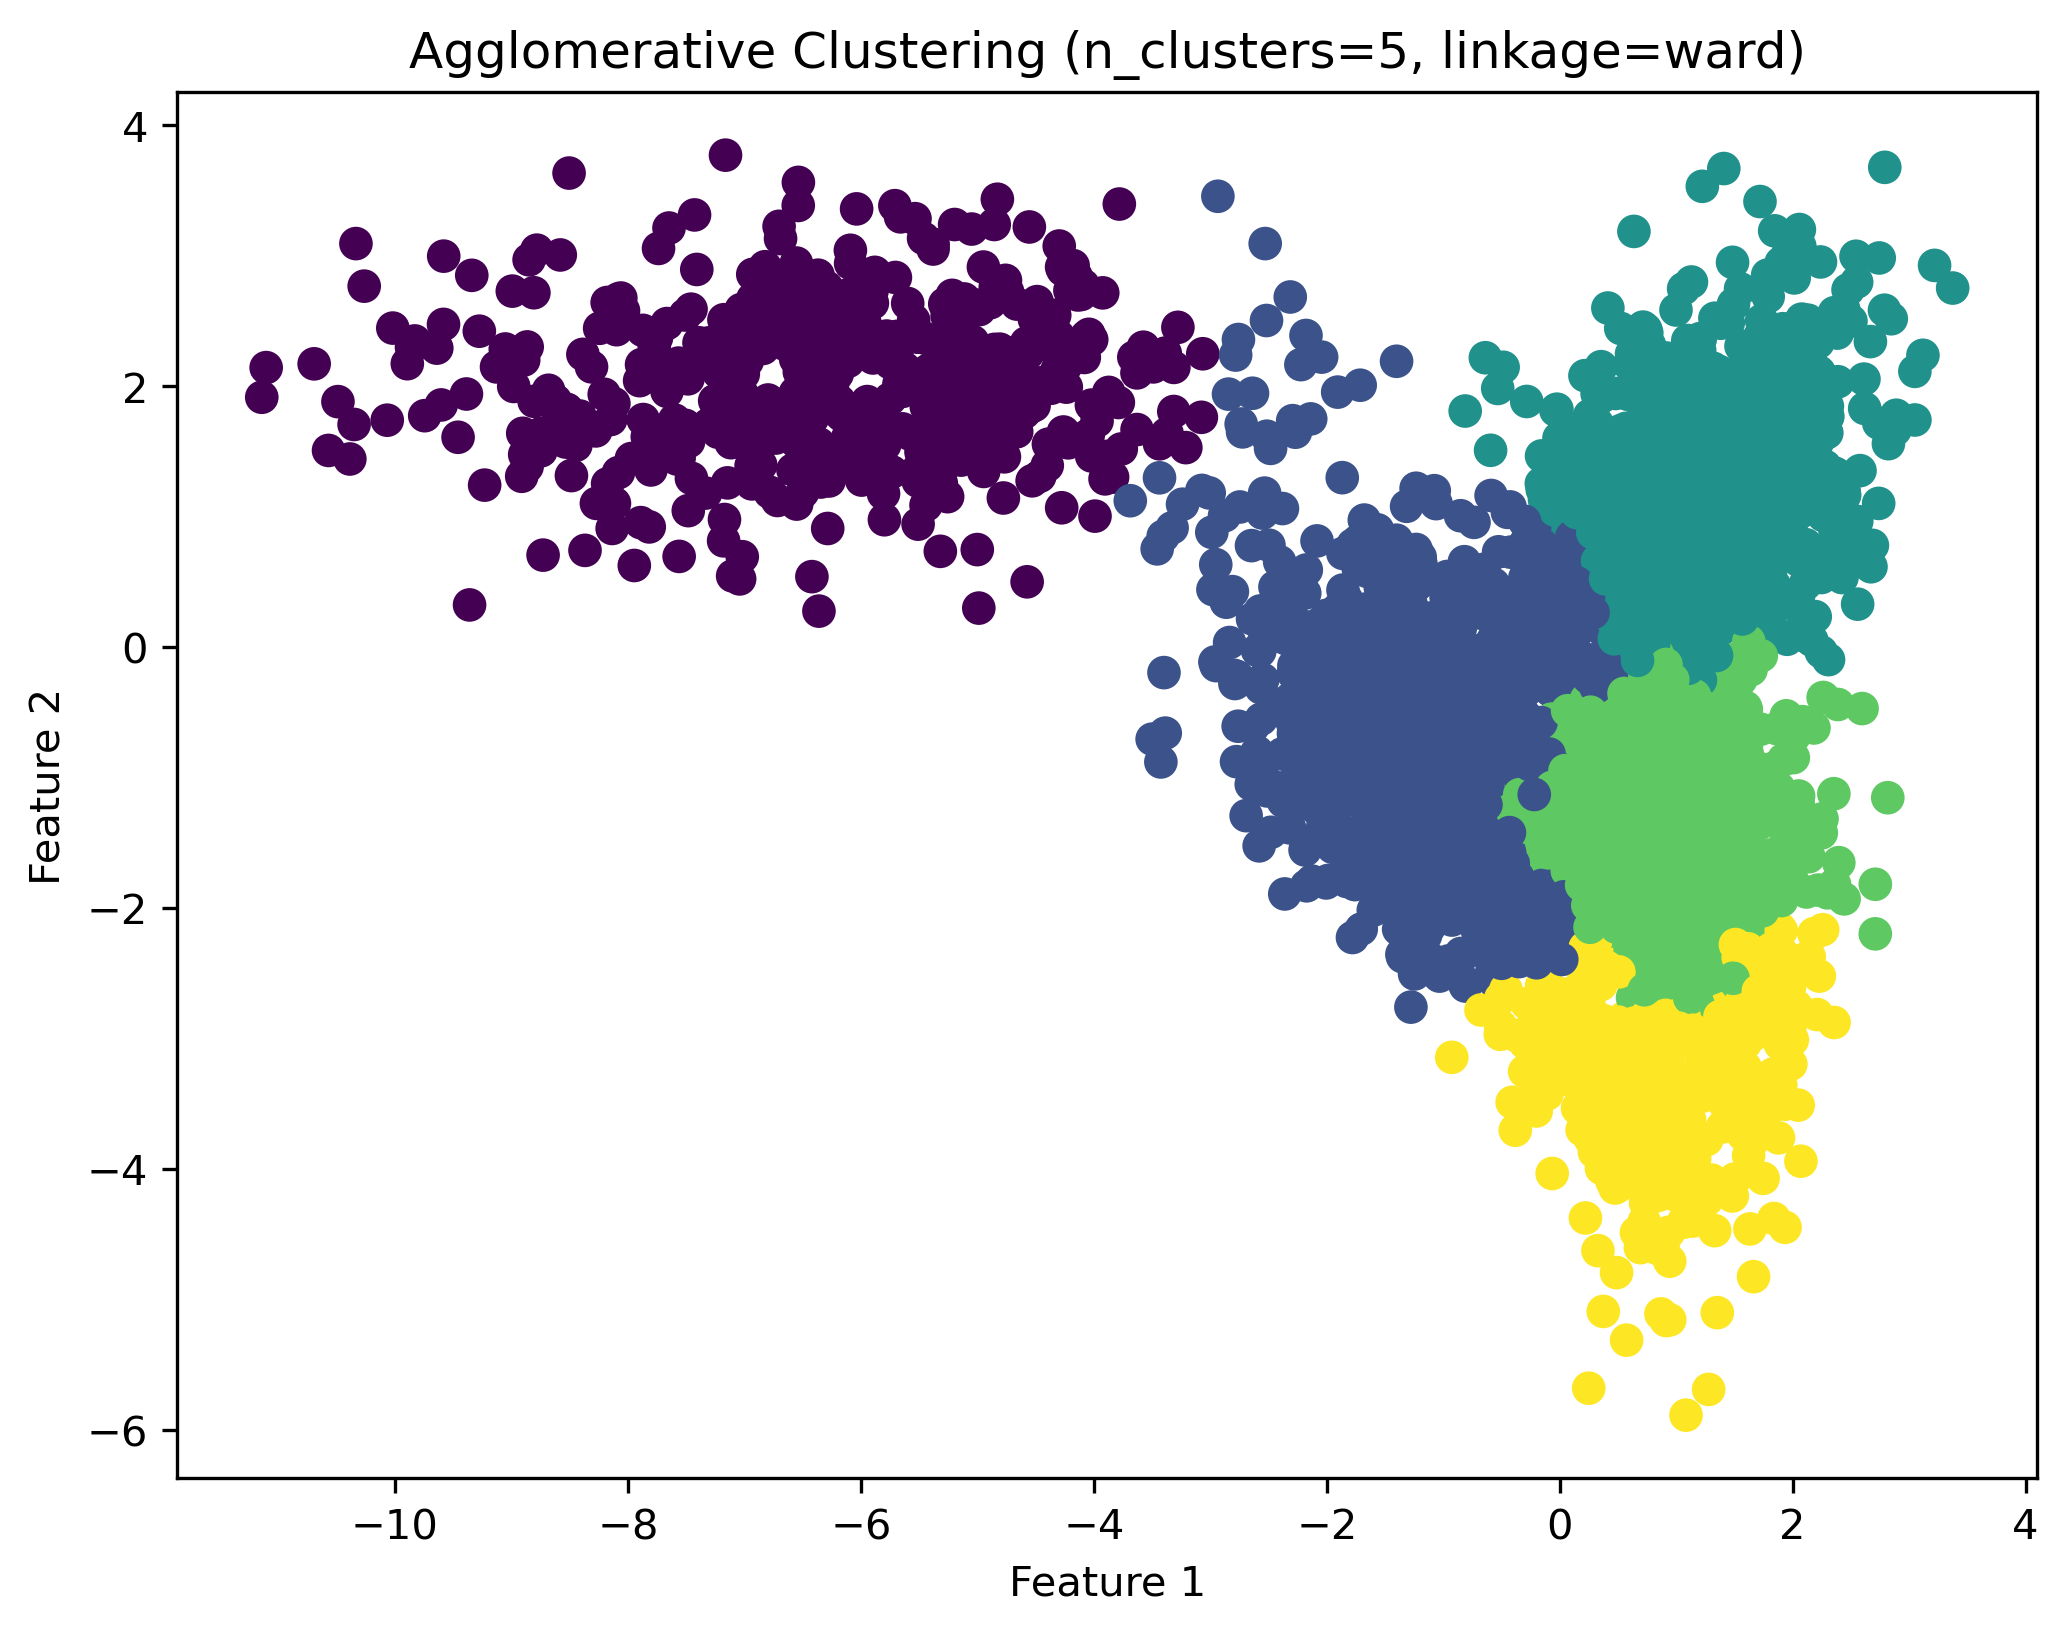
\includegraphics[width=\textwidth]{figures/agglomerative_scatter_d0.png}
        \caption{Dataset 1 (2D)}
        \label{fig:agglo_2d}
    \end{subfigure}
    \begin{subfigure}[b]{0.45\textwidth}
        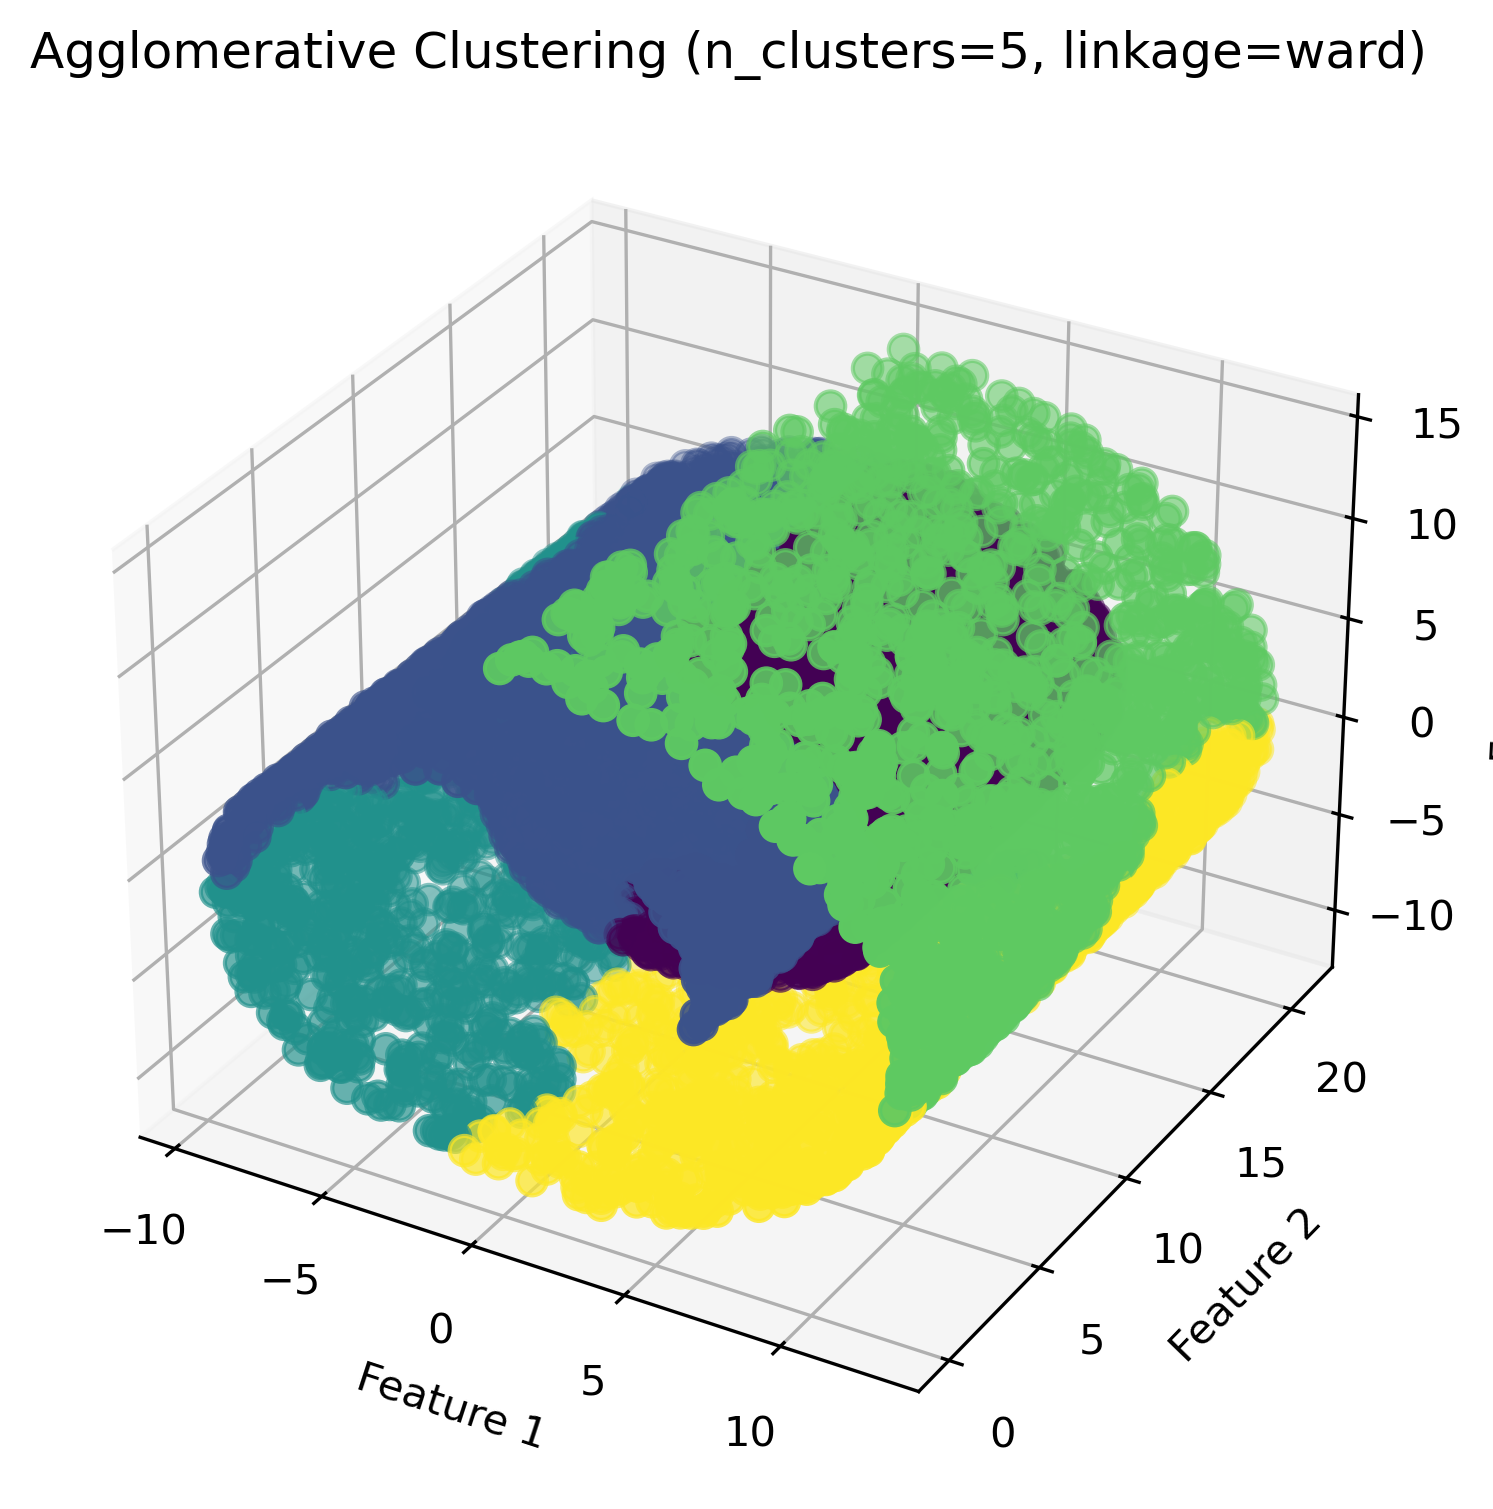
\includegraphics[width=\textwidth]{figures/agglomerative_scatter_d1.png}
        \caption{Dataset 2 (3D)}
        \label{fig:agglo_3d}
    \end{subfigure}
    \caption{Scatterplots for agglomerative clustering}
    \label{fig:agglo_scatterplots}
\end{figure}

\section{Discussion}
\subsection{Lloyd’s Algorithm}
For Dataset 1, the elbow method suggests that the optimal number of clusters is around $k=5$, as the clustering cost begins to plateau after this point. For Dataset 2, the elbow is less pronounced, but $k=8$ appears to be a reasonable choice.

\subsection{Hierarchical Agglomerative Clustering}
The dendrograms for both datasets reveal a hierarchical structure. For Dataset 1, the dendrogram suggests a natural cut-off at 4 clusters, consistent with the k-means results. For Dataset 2, the dendrogram indicates a more complex structure, with a potential cut-off at 5 clusters.

\subsection{Comparison of Methods}
\begin{itemize}
    \item \textbf{Stability}: Lloyd’s algorithm is sensitive to initialization, while hierarchical clustering is deterministic but computationally expensive for large datasets.
    \item \textbf{Accuracy}: Both methods produced similar results for Dataset 1, but hierarchical clustering provided more nuanced insights for Dataset 2 due to its ability to capture hierarchical relationships.
    \item \textbf{Computational Complexity}: Lloyd’s algorithm is faster for large datasets, while hierarchical clustering is more suitable for smaller datasets or when hierarchical relationships are of interest.
\end{itemize}

\section{Conclusion}
The experiments demonstrate that both Lloyd’s algorithm and hierarchical agglomerative clustering are effective for identifying clusters in the datasets. The choice of method depends on the dataset size and the need for hierarchical insights. Future work could explore hybrid approaches or alternative clustering algorithms such as DBSCAN for datasets with varying densities.

\section*{References}
\begin{itemize}
    \item Lecture slides from Seng 474: Data Mining.
    \item Scikit-learn documentation: \url{https://scikit-learn.org/stable/}
    \item SciPy documentation: \url{https://docs.scipy.org/doc/scipy/reference/cluster.hierarchy.html}
\end{itemize}

\end{document}